\documentclass[10pt]{beamer}
\usepackage[ngerman]{babel}
\usepackage[utf8x]{inputenc}
\usepackage{amsmath, amsfonts, amssymb}
\usepackage{tikz}
\usepackage{pgfplots}
\usepackage{xcolor}
\usepackage{subcaption}
\usepackage{trfsigns}
\usepackage{wasysym}

% todo: bold

\usetheme{Luebeck}
\useinnertheme{rounded}
\usefonttheme{professionalfonts}
\setbeamercovered{transparent}
\beamertemplatenavigationsymbolsempty
\setbeamertemplate{footline}{%
  \begin{beamercolorbox}[wd = 0.5\textwidth, ht = 3ex, dp = 1.5ex, leftskip = .5em,
      rig htskip = .5em]{author in head/foot}%
    \usebeamerfont{author in head/foot}%
    \insertframenumber/\inserttotalframenumber\hfill\insertshortauthor%
  \end{beamercolorbox}%
  \vspace*{-4.5ex}\hspace*{0.5\textwidth}%
  \begin{beamercolorbox}[wd = 0.5\textwidth, ht = 3ex, dp = 1.5ex, left, leftskip = .5em]{title in head/foot}%
    \usebeamerfont{title in head/foot}%
    \insertshorttitle%
\end{beamercolorbox}}

\newcommand*{\ClipSep}{0.3cm}%

\renewcommand{\arraystretch}{1.3}

\title{Multi-Gigabit Complex Sub-Nyquist Sampling SDR for 60 GHz}
\subtitle{Master Thesis at the Telecommunications Circuits Lab, EPFL}
\author{Lorenz Koestler $ < $lorenzk@ee.ethz.ch$ > $}
\date[1.9..2013]{1. September 2014}


\setbeamercolor{author}{fg=white}
\setbeamercolor{date}{fg=white}


\addtobeamertemplate{title page}{%
  \vspace{-1.5cm}
}{}

\newcommand{\mc}[2]{\multicolumn{#1}{c|}{#2}}

\begin{document}

{
  \usebackgroundtemplate{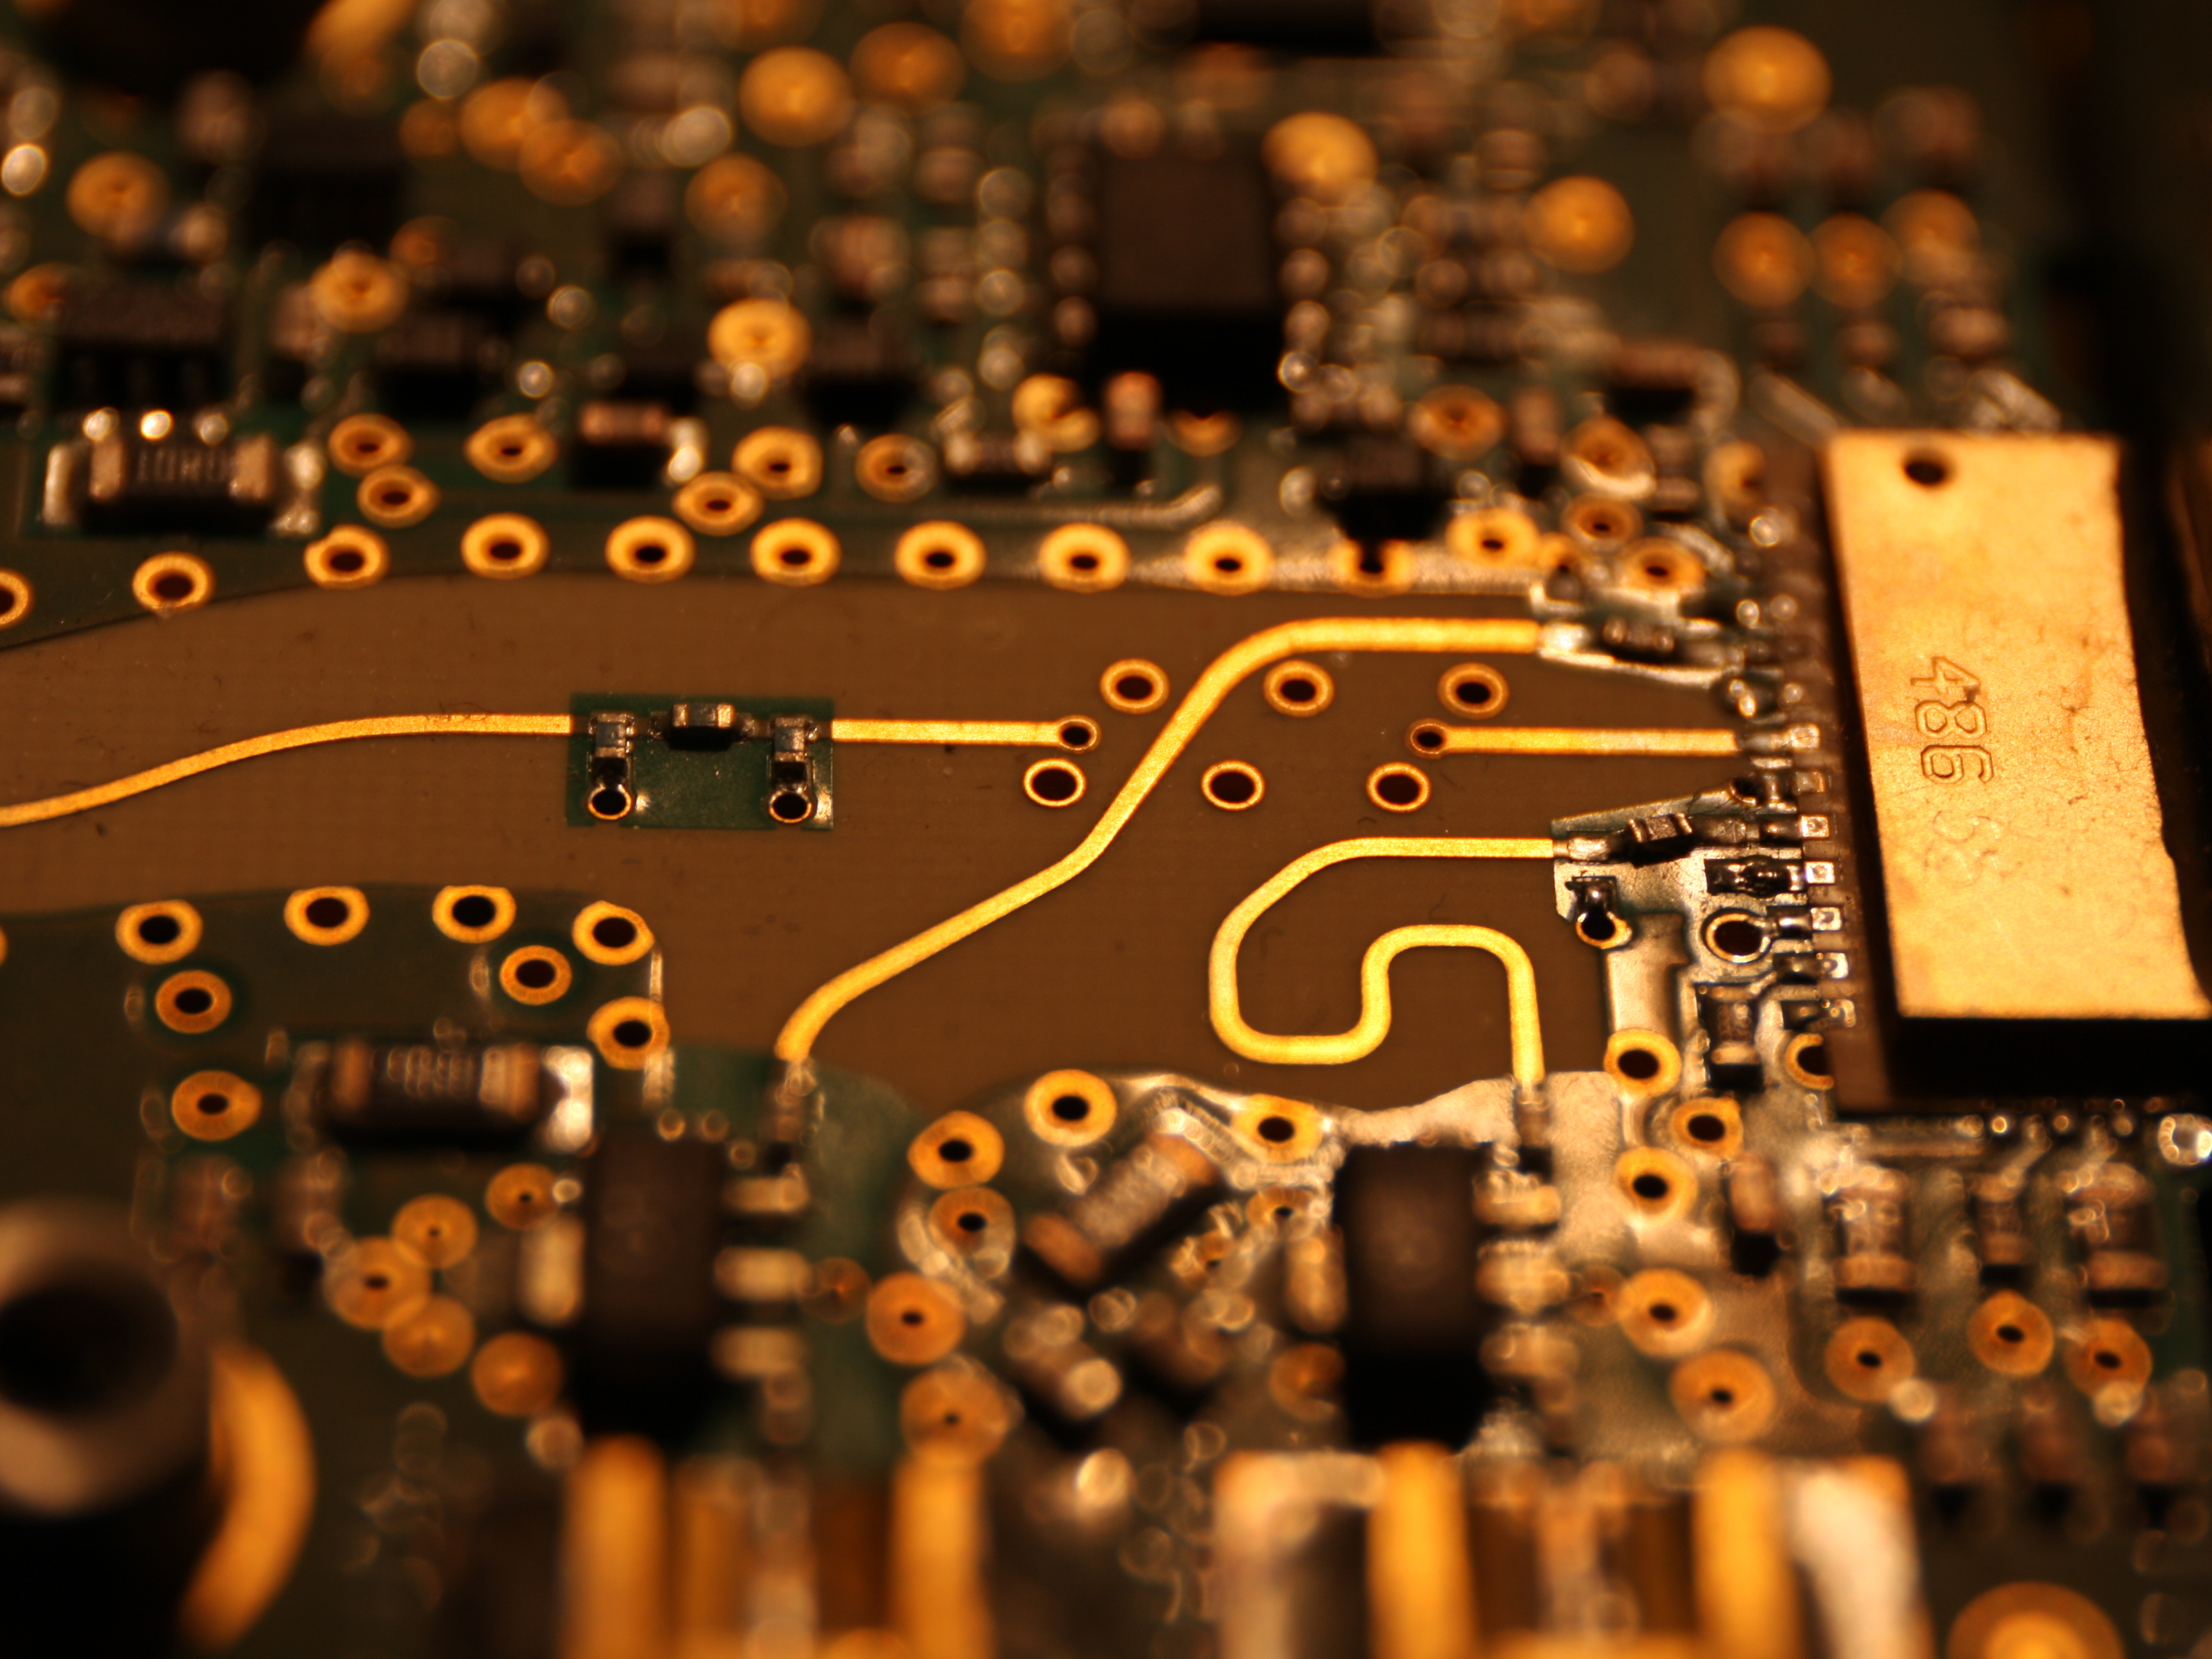
\includegraphics[width=\paperwidth]{pictures/back}}
  \begin{frame}
    \titlepage

    {\color{white}
      Advisors: \\
      Nicholas Preyss $ < $\href{mailto:nicholas.preyss@epfl.ch}{nicholas.preyss@epfl.ch}$ > $ \\
    }
  \end{frame}
}

\begin{frame}{Introduction}
  \begin{itemize}
  \item Mobile communication systems became ubiquitous
  \item Essential importance that network throughput increases
    exponentially
  \item Higher spectral efficiency (channel allocation, MIMO etc.) is possible
  \item Move to new frequency bands to increase bandwidth
  \item 60 GHz band offers two orders of magnitude higher bandwidth
  \item Possibility for big antenna arrays on small surface
  \item High spatial selectivity allows reusage of channel
  \end{itemize}
  \begin{block}{New Applications:}
    \begin{itemize}
    \item Lossless, uncompressed HD video streams
    \item High density cell networks (5G)
    \item Multiplication of WiFi troughput
    \end{itemize}
  \end{block}
\end{frame}

\begin{frame}{Objectives}
  \begin{columns}[T]
    \begin{column}{.6\textwidth}
      \begin{itemize}
      \item Analyze suitable receiver designs
      \item Setup of a versatile simulation and measurement framework
      \item Characterize communication parameters
      \item Show that high modulation rates are possible
      \item Find performance limiting impairments for 60 GHz communication systems
      \end{itemize}
    \end{column}
    \begin{column}{.4\textwidth}
      \begin{tikzpicture}
        \node [inner sep=0pt] at (0,0) {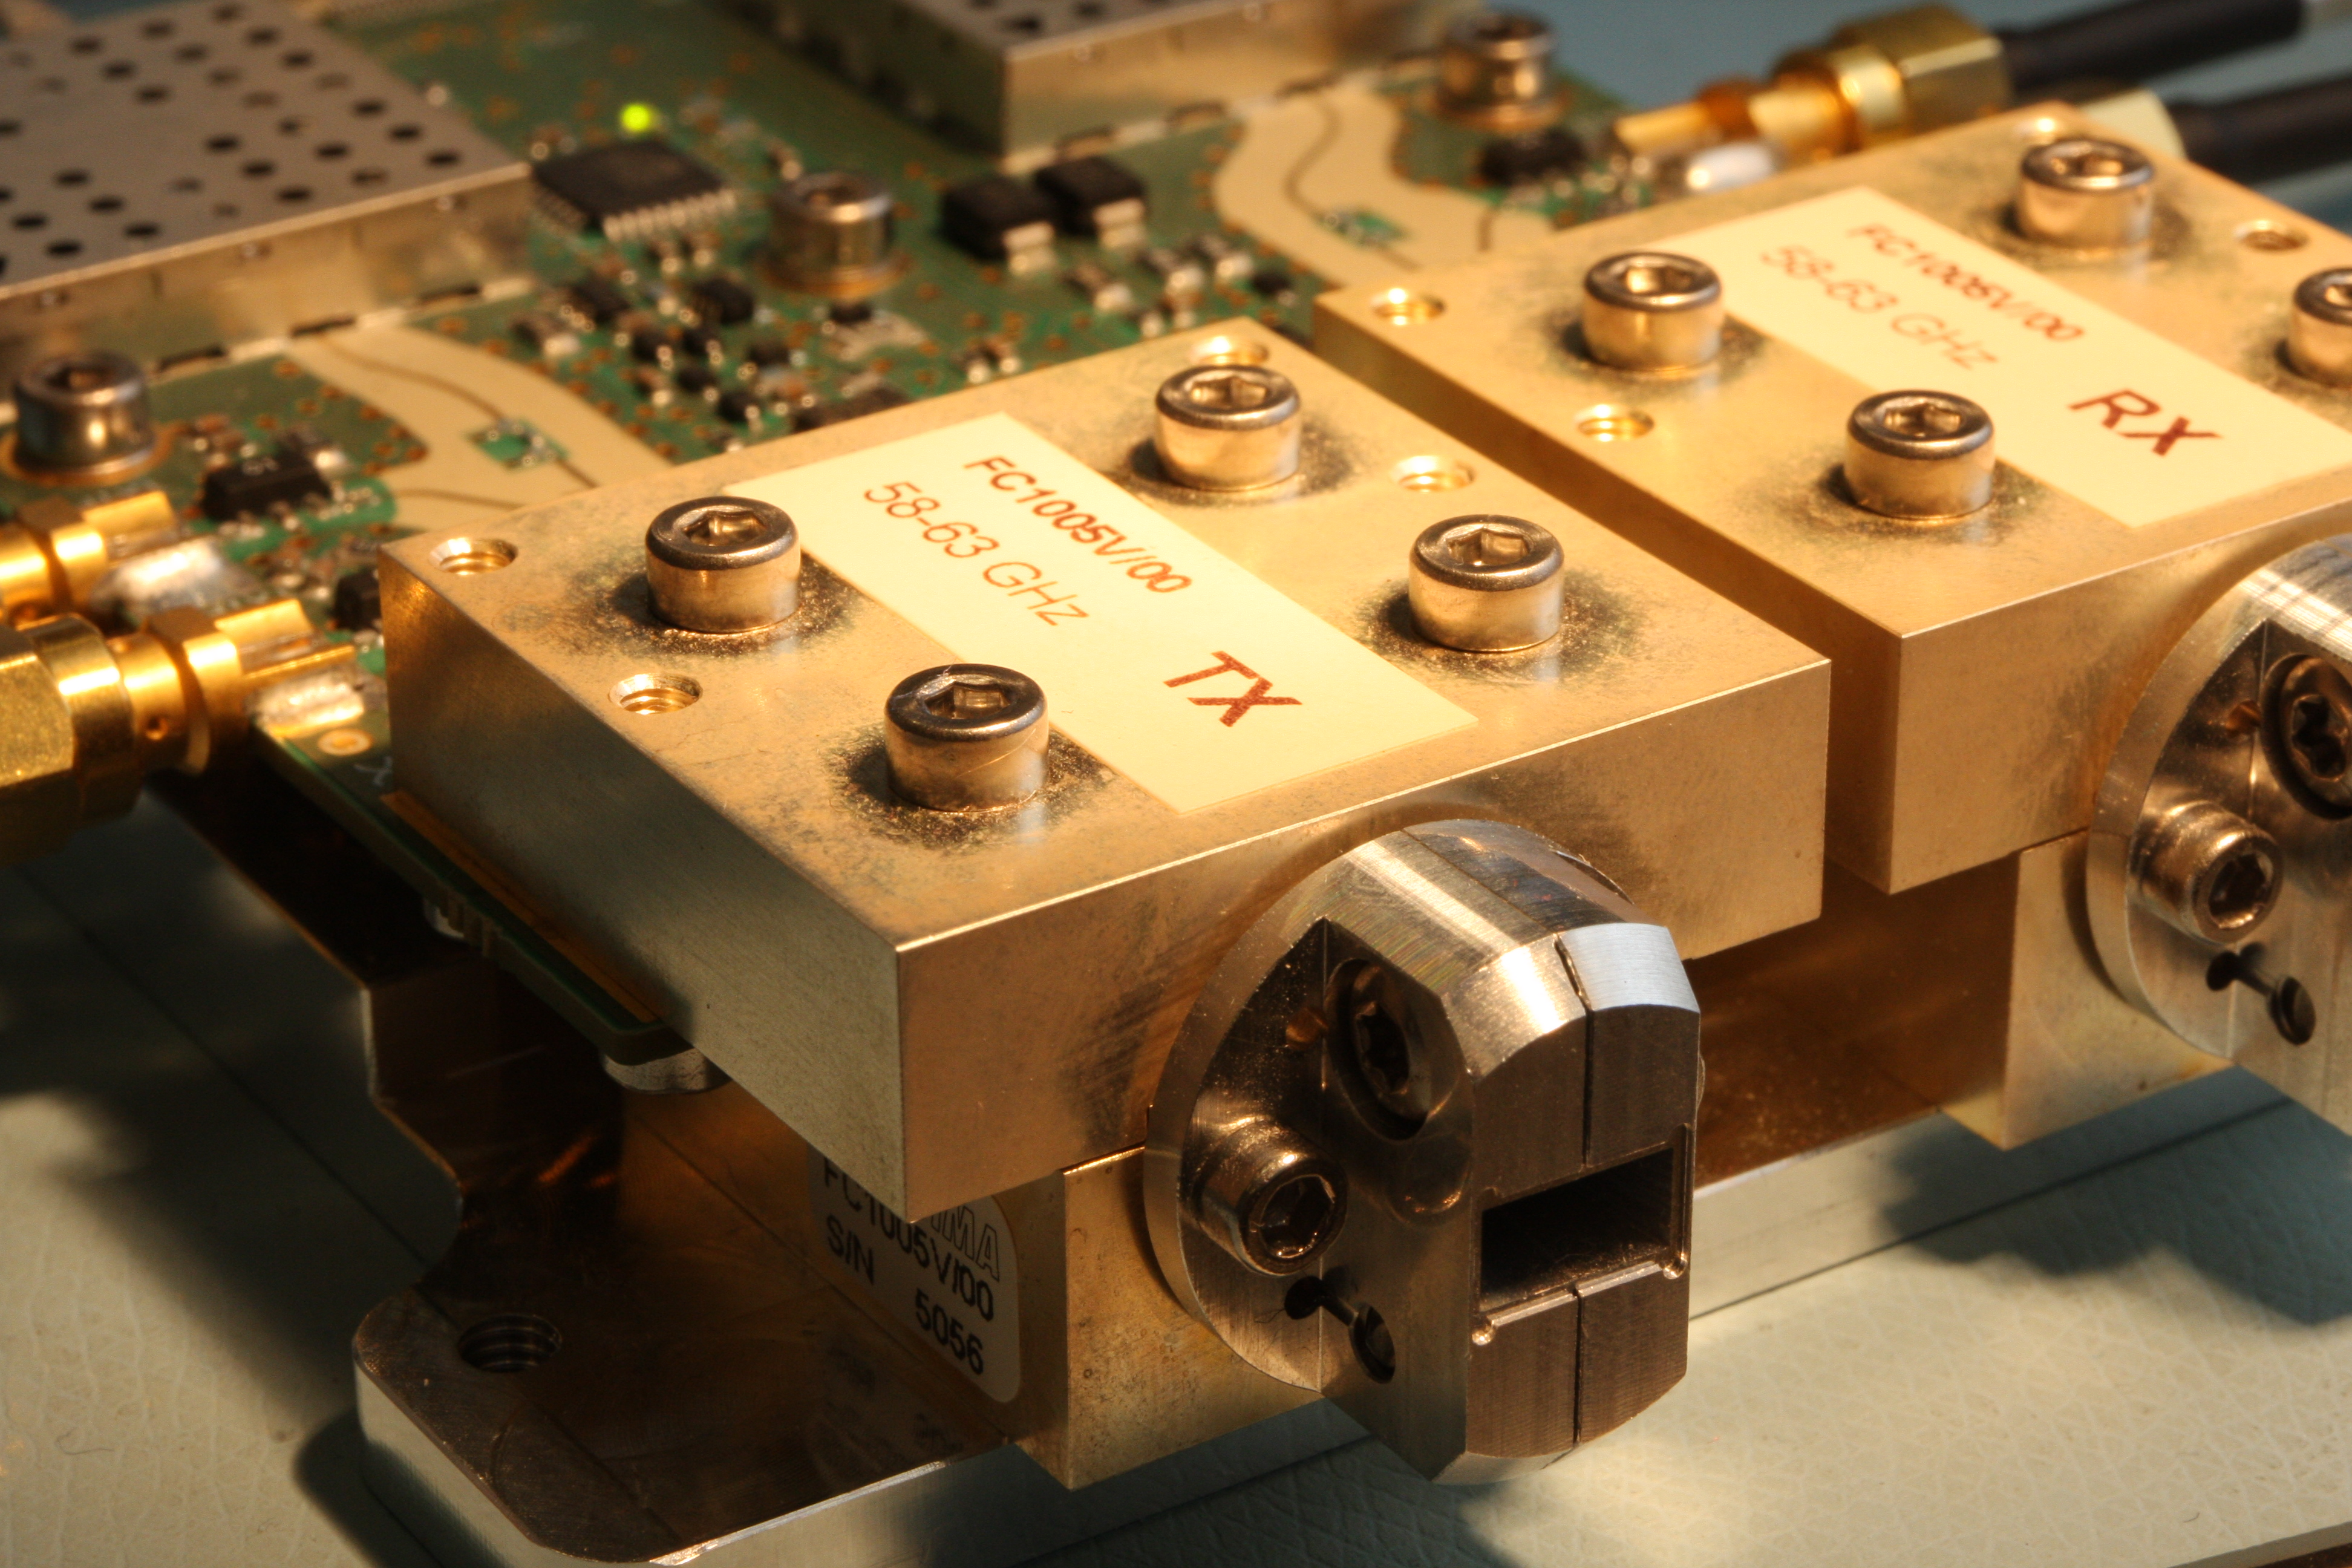
\includegraphics[width=\textwidth]{pictures/sivers_ant}};
        \draw [white, rounded corners=\ClipSep, line width=\ClipSep]
        (current bounding box.north west) --
        (current bounding box.north east) --
        (current bounding box.south east) --
        (current bounding box.south west) -- cycle
        ;
      \end{tikzpicture}
    \end{column}
  \end{columns}
\end{frame}

\begin{frame}{Receiver Designs}
  \begin{columns}[T]
    \begin{column}{.5\textwidth}
      \begin{block}{Goal}
        \begin{itemize}
        \item Digitize the channel of interest with as high as possible
          dynamic range
        \item Suppress influence of other channels
        \end{itemize}
      \end{block}
      \begin{tikzpicture}
        \node [inner sep=0pt] at (0,0)
              {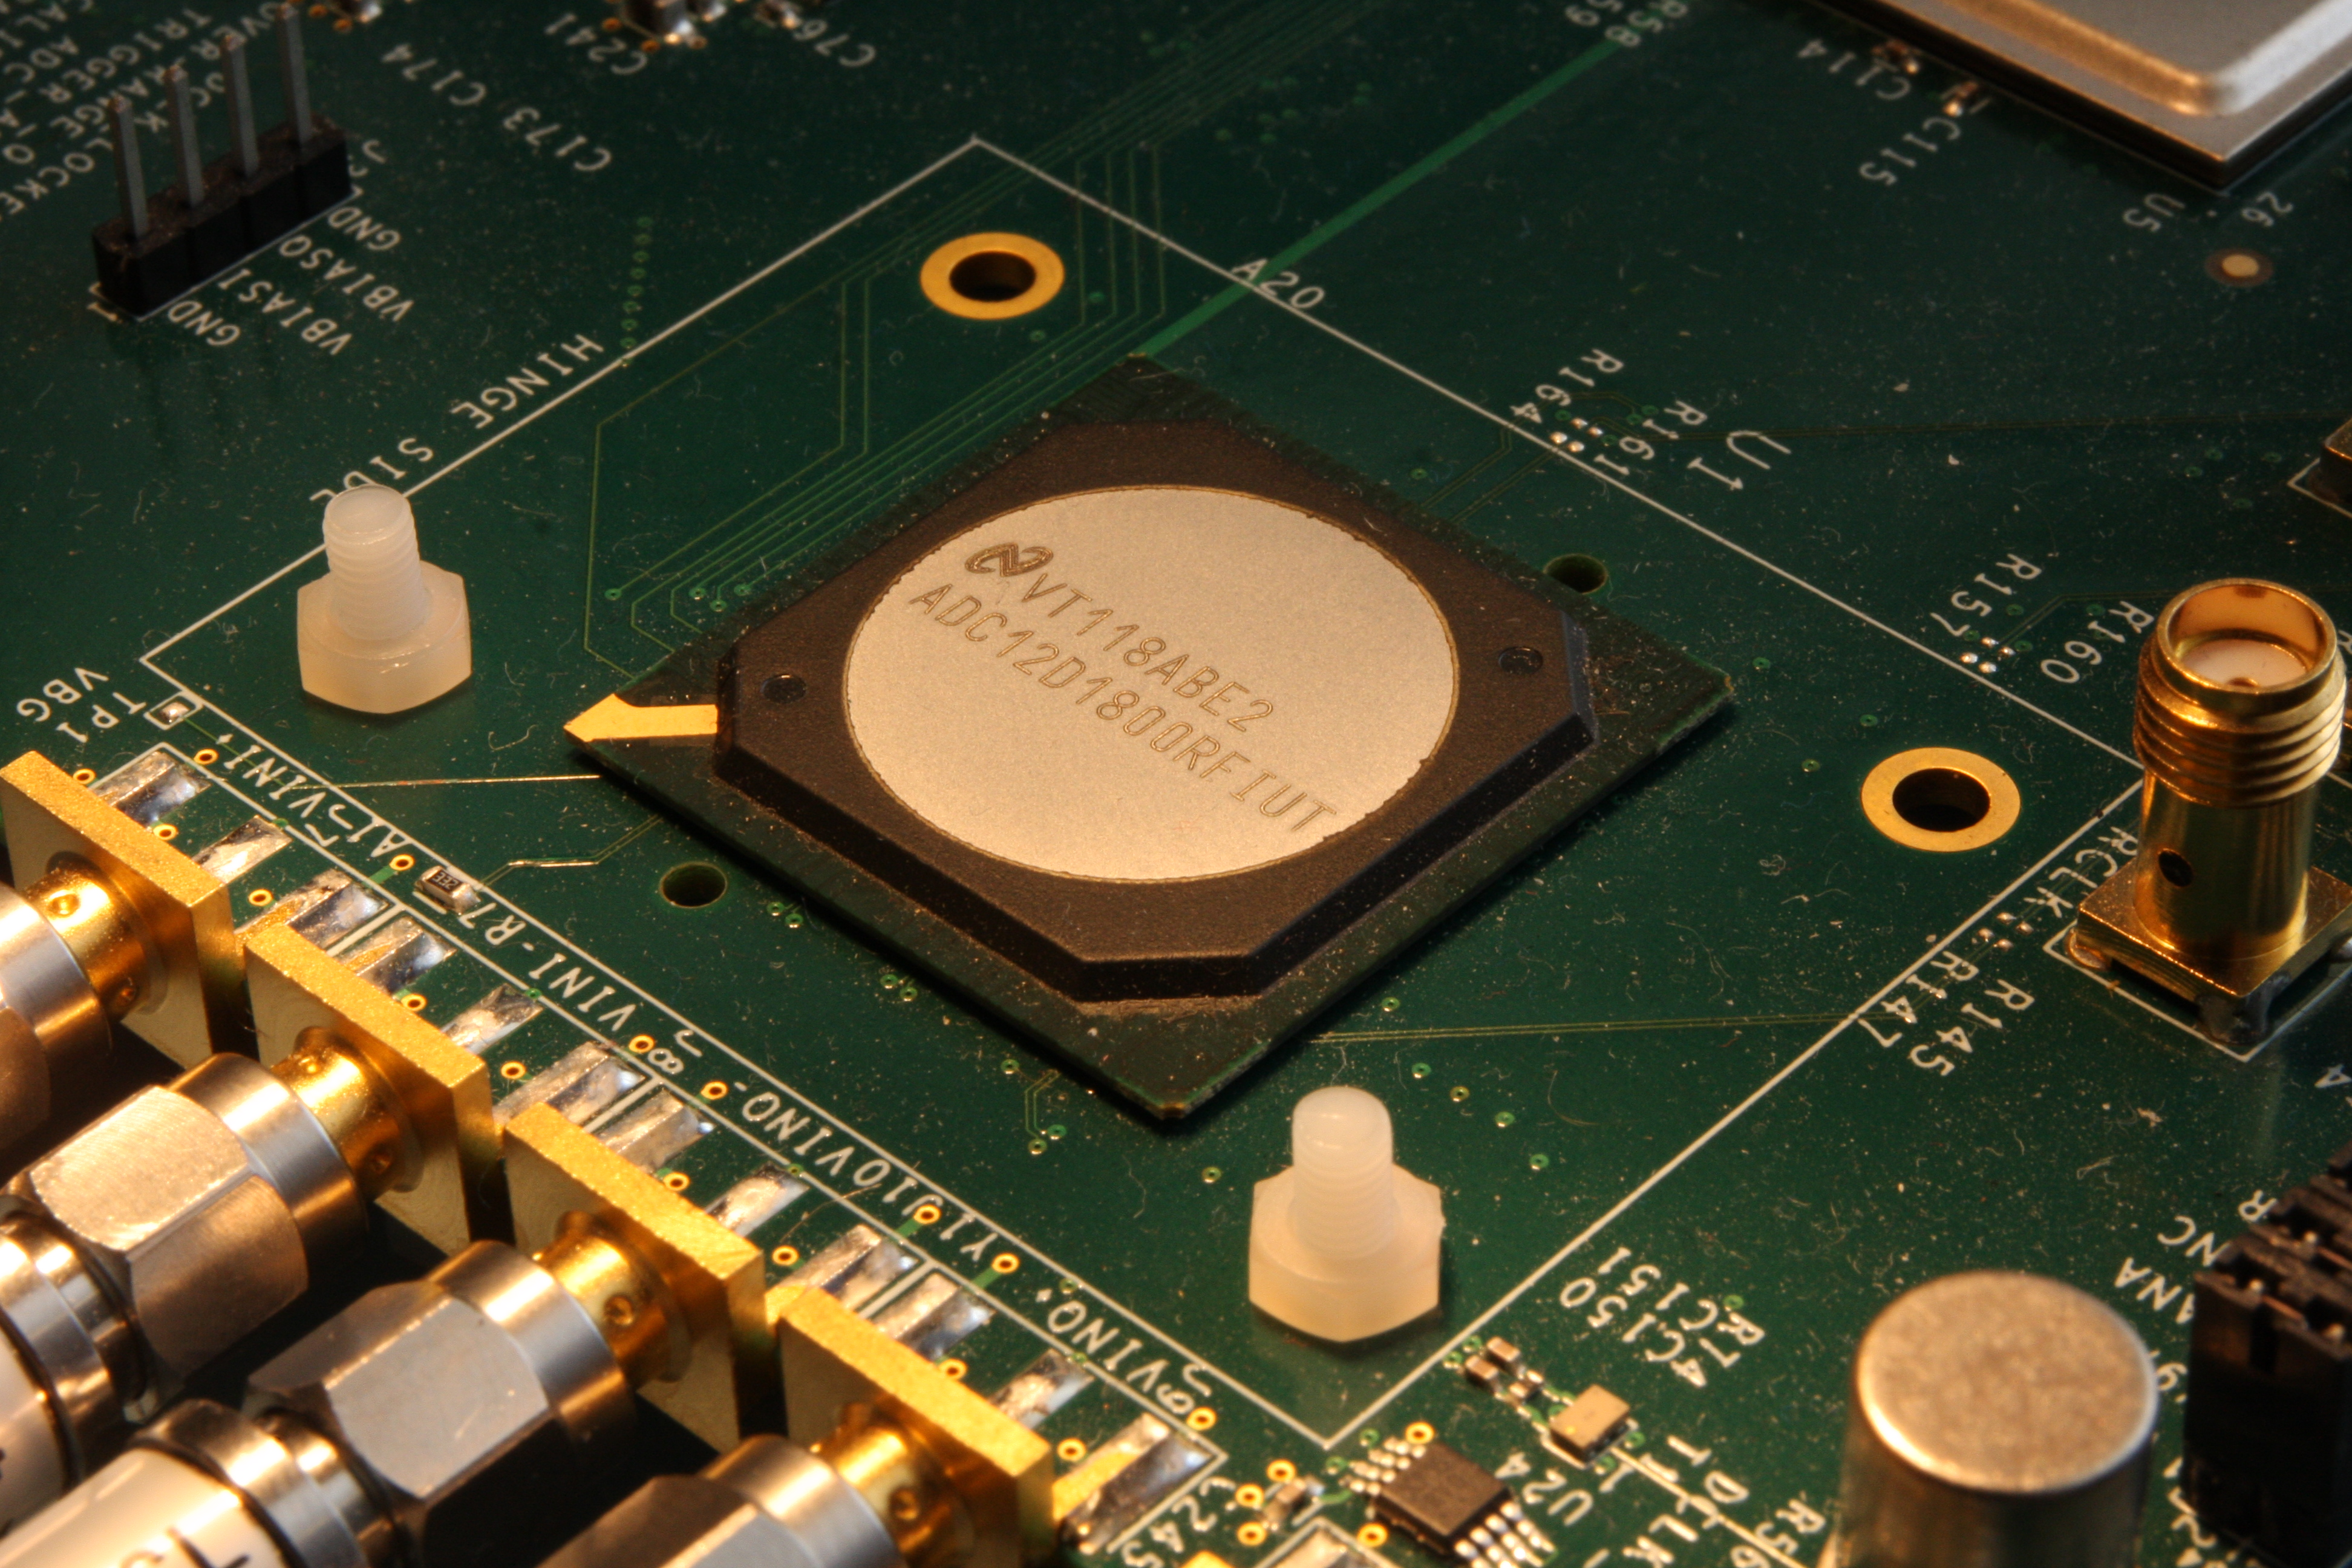
\includegraphics[width=\textwidth]{pictures/adc}};
              \draw [white, rounded corners=\ClipSep, line
                width=\ClipSep] (current bounding box.north west) --
              (current bounding box.north east) -- (current bounding
              box.south east) -- (current bounding box.south west) --
              cycle ;
      \end{tikzpicture}
    \end{column}
    \begin{column}{.5\textwidth}
      \begin{block}{Challenge}
        \begin{itemize}
        \item Many component restrictions exist
        \item Channel width is as high as the available ADC sampling
          speeds $\rightarrow$ Oversampling is not easily possible
        \item Channel bandwidth covers most of the usable frequency
          range of components
          (eg. 1.8 GHz wide channel on IF center frequency of 1 GHz)
        \item[$\Rightarrow$] {\bf Frequency planning is more complicated}
        \end{itemize}
      \end{block}
    \end{column}
  \end{columns}
\end{frame}

\begin{frame}{Direction Conversion / High IF Receiver}
  \begin{columns}[T]
    \begin{column}{.6\textwidth}
      \vspace{5mm}
      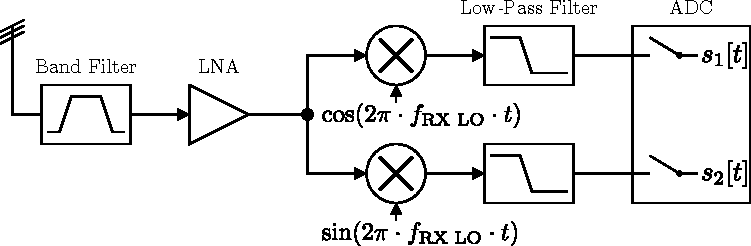
\includegraphics[width=\textwidth]{figures/rx_4_bd}
    \end{column}
    \begin{column}{.4\textwidth}
      \begin{block}{Direction Conversion}
        \begin{itemize}
        \item Most common digital RX architecture
        \item[\frownie] 60 GHz RF frontend does not go below 1~GHz
        \end{itemize}
      \end{block}
    \end{column}
  \end{columns}
  \vspace{4ex}
  \begin{columns}[T]
    \begin{column}{.6\textwidth}
      \vspace{5mm}
      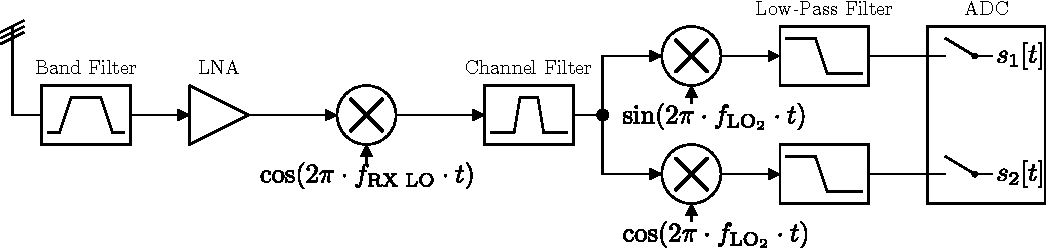
\includegraphics[width=\textwidth]{figures/rx_0_bd}
    \end{column}
    \begin{column}{.4\textwidth}
      \begin{block}{High IF Receiver}
        \begin{itemize}
        \item DC-Block blocks part of signal
        \item[\frownie] Second IF would have to be at 8~GHz
        \end{itemize}
      \end{block}
    \end{column}
  \end{columns}
\end{frame}

\begin{frame}{High IF Receiver}
  \begin{columns}[T]
    \begin{column}{.6\textwidth}
      \vspace{5mm}
      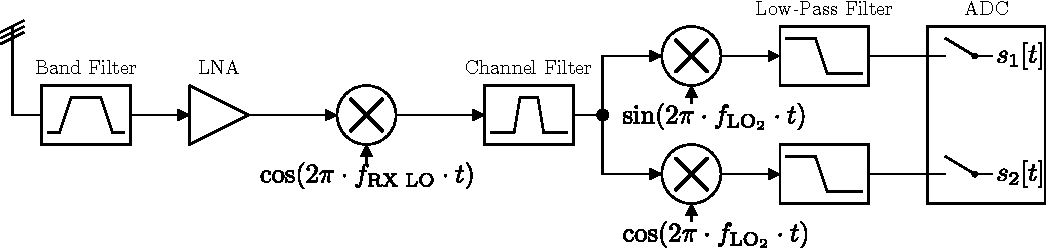
\includegraphics[width=\textwidth]{figures/rx_0_bd}
    \end{column}
    \begin{column}{.4\textwidth}
      \begin{block}{High IF Receiver}
        \begin{itemize}
        \item DC-Block blocks part of signal
        \item[\frownie] Second IF would have to be at 8~GHz
        \end{itemize}
      \end{block}
    \end{column}
  \end{columns}
  \vspace{1cm}
  \begin{columns}[T]
    \begin{column}{.5\textwidth}
      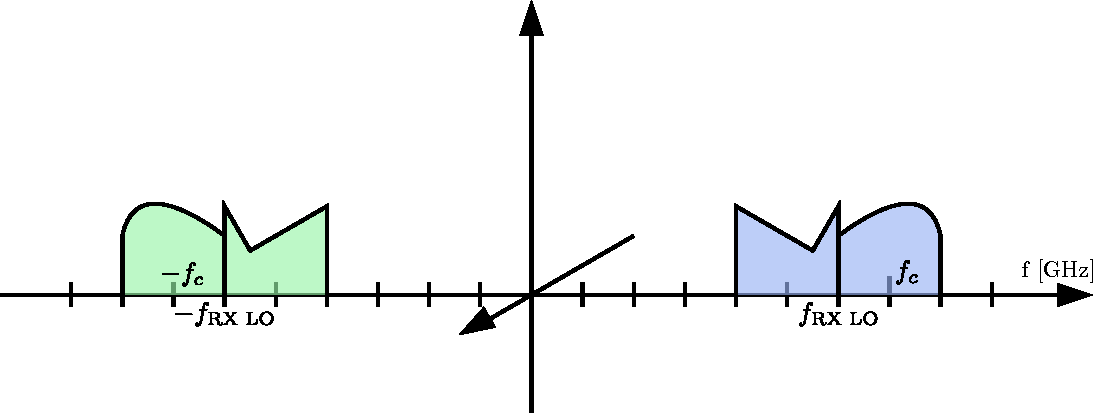
\includegraphics[width=\textwidth]{figures/rx_rf_0_freq_s}
    \end{column}
    \begin{column}{.5\textwidth}
      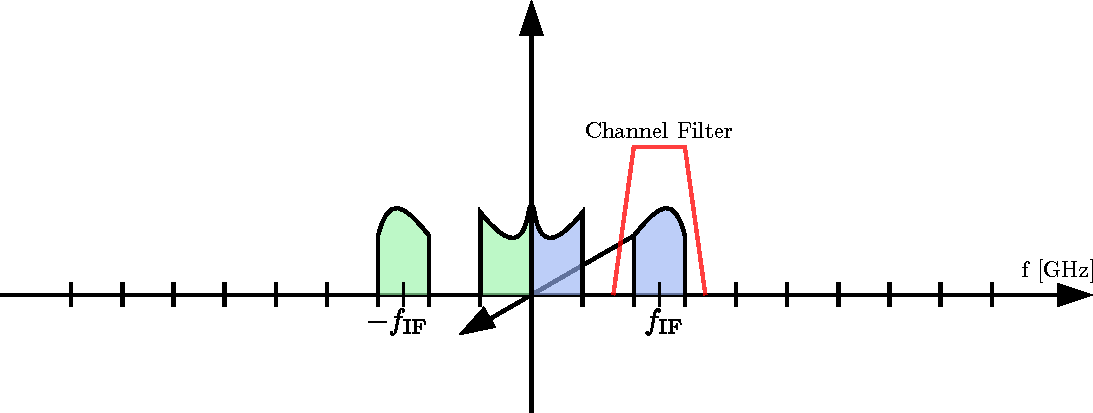
\includegraphics[width=\textwidth]{figures/rx_rf_0_freq_i}
    \end{column}
  \end{columns}
  \vspace{11ex}
\end{frame}

\begin{frame}{Chosen Design: \newline Quadrature IF Sub-Nyquist Sampling Receiver}
  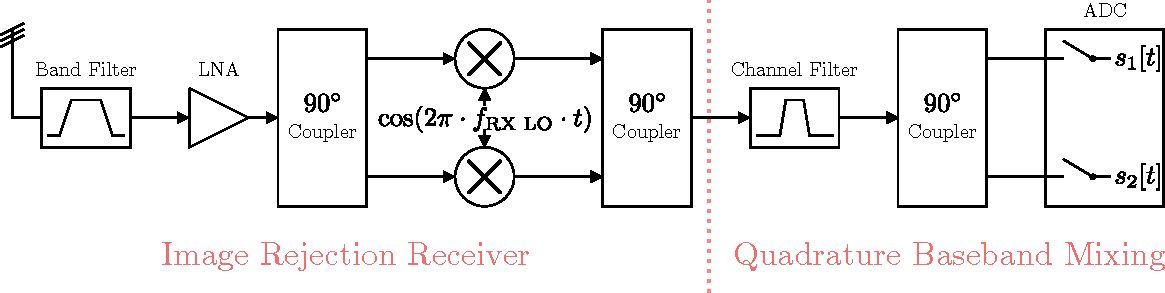
\includegraphics[width=\textwidth]{figures/rx_3_bd} \\
  \vspace{5mm}
  \begin{block}{Advantages}
    \begin{itemize}
    \item Image rejection relaxes requirements on preselection
    \item Quadrature sub-Nyquist sampling allows for low IF
    \end{itemize}
  \end{block}
\end{frame}

\begin{frame}{$90^\circ$ Coupler / Hilbert Transform}
  \begin{columns}[T]
    \begin{column}{.5\textwidth}
      \begin{block}{Time Domain}
        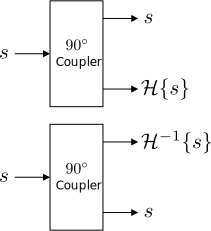
\includegraphics[width=\textwidth]{figures/90deg_coupler_hilbert}
      \end{block}
    \end{column}
    \begin{column}{.5\textwidth}
      \begin{block}{Frequency Domain}
        \centering
        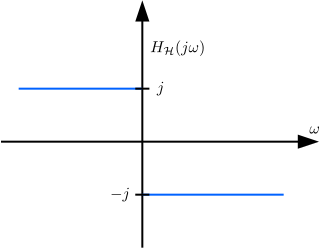
\includegraphics[width=0.7\textwidth]{figures/hilbert}
      \end{block}
      \centering
      \begin{tikzpicture}
        \node [inner sep=0pt] at (0,0) {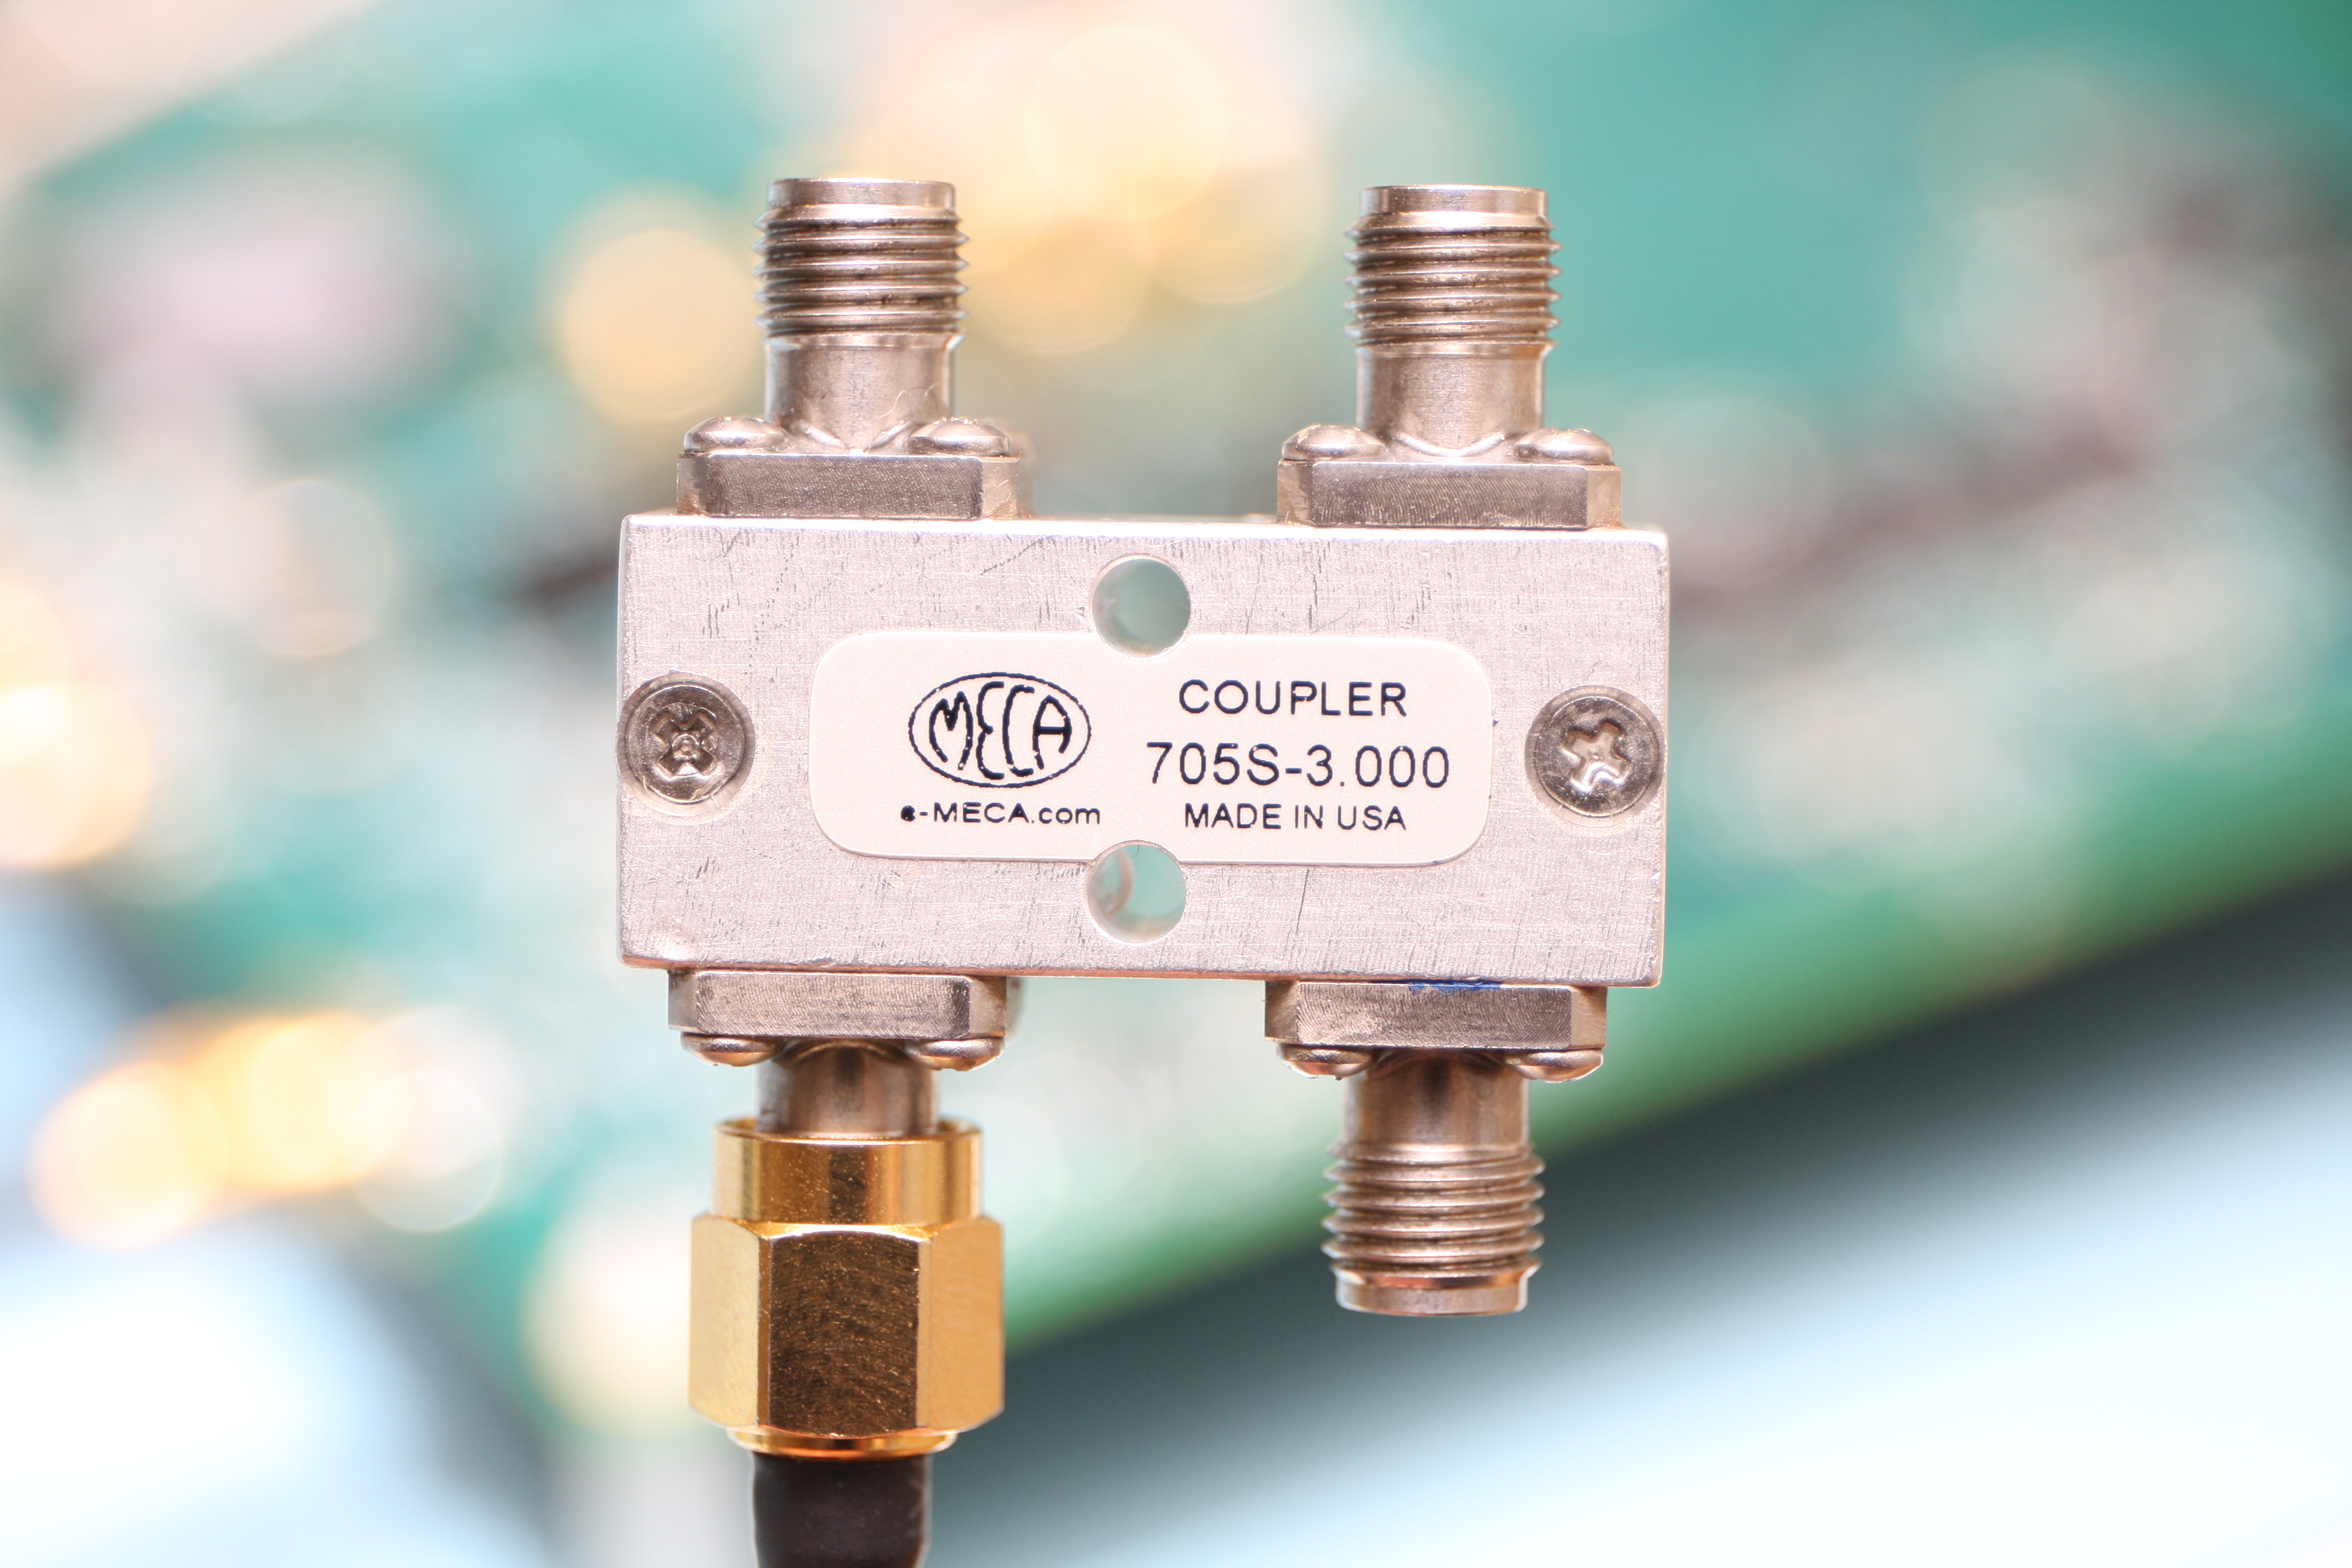
\includegraphics[width=0.9\textwidth]{pictures/90deg}};
        \draw [white, rounded corners=\ClipSep, line width=\ClipSep]
        (current bounding box.north west) --
        (current bounding box.north east) --
        (current bounding box.south east) --
        (current bounding box.south west) -- cycle
        ;
      \end{tikzpicture}
    \end{column}
  \end{columns}
\end{frame}

\begin{frame}{Image Rejection using $90^\circ$ Couplers}
  \only<1>{
    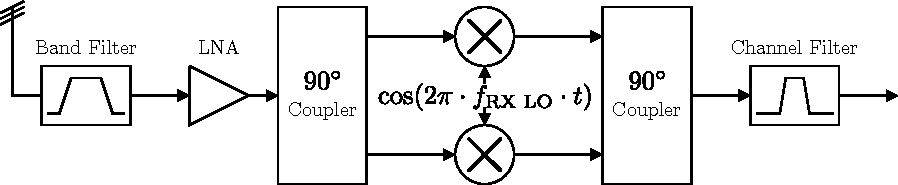
\includegraphics[width=\textwidth]{figures/rx_rf_1_bd}
    \vspace{4mm}
  }

  \only<1-2>{
    \begin{columns}[T]
      \begin{column}{.5\textwidth}
        {\color{blue} Step 1:}
        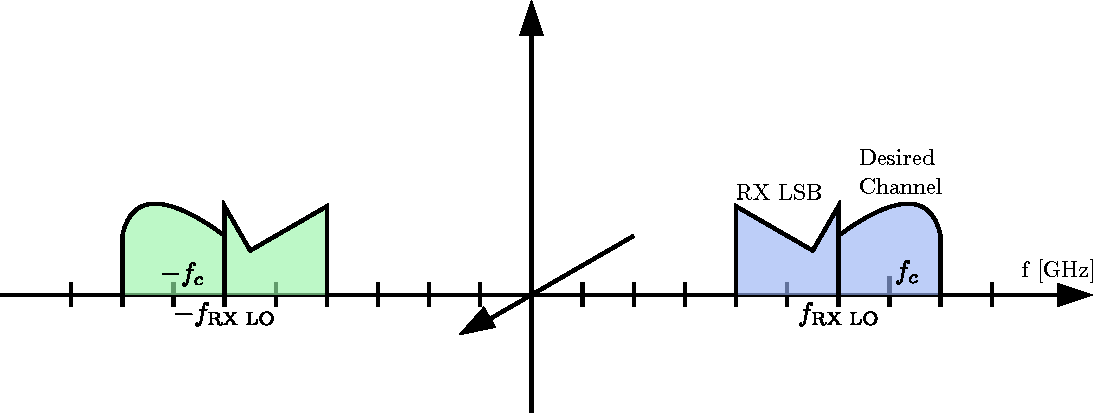
\includegraphics[width=\textwidth]{figures/rx_rf_1_freq_s}
        \vspace{-3mm}
        \[r(t)\]
      \end{column}
      \begin{column}{.5\textwidth}
        \vspace{1eM}
        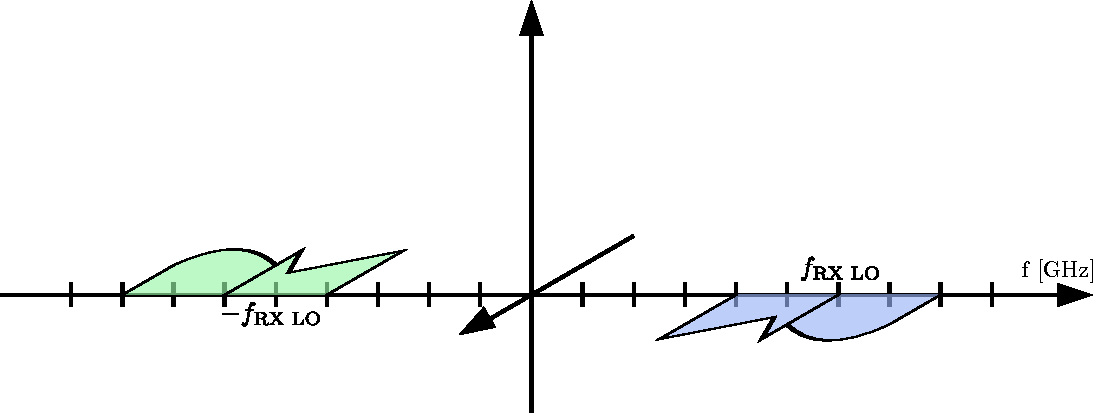
\includegraphics[width=\textwidth]{figures/rx_rf_1_freq_Hs}
        \vspace{-3mm}
        \[\mathcal{H}^{-1}\{r\}(t)\]
      \end{column}
    \end{columns}
  }

  \only<2-3>{
    \vspace{5mm}
    \begin{columns}[T]
      \begin{column}{.5\textwidth}
        {\color{blue} Step 2:}
        \vspace{5mm}
        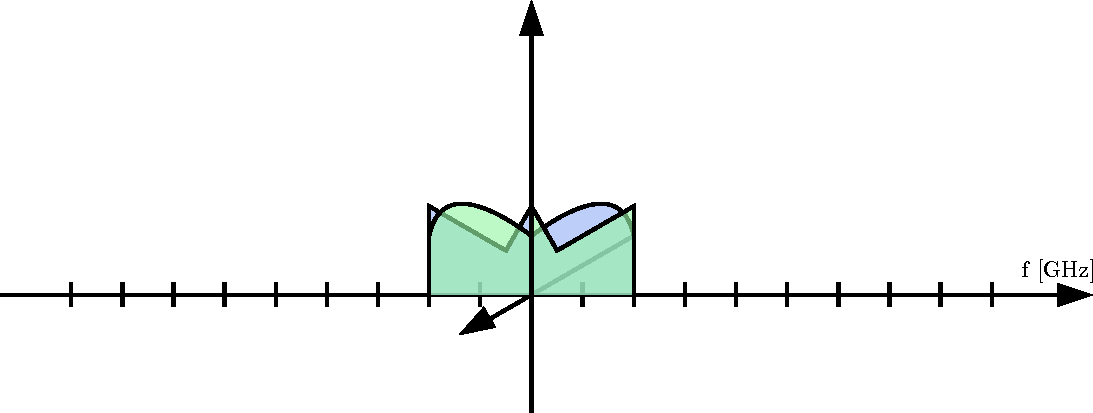
\includegraphics[width=\textwidth]{figures/rx_rf_1_freq_a}
        \vspace{-8mm}
        \[a(t) = \text{LP}\{r(t) \cdot \cos(2\pi \cdot f_{\text{RX LO}} \cdot t)\}\]
      \end{column}
      \begin{column}{.5\textwidth}
        \vspace{1eM}
        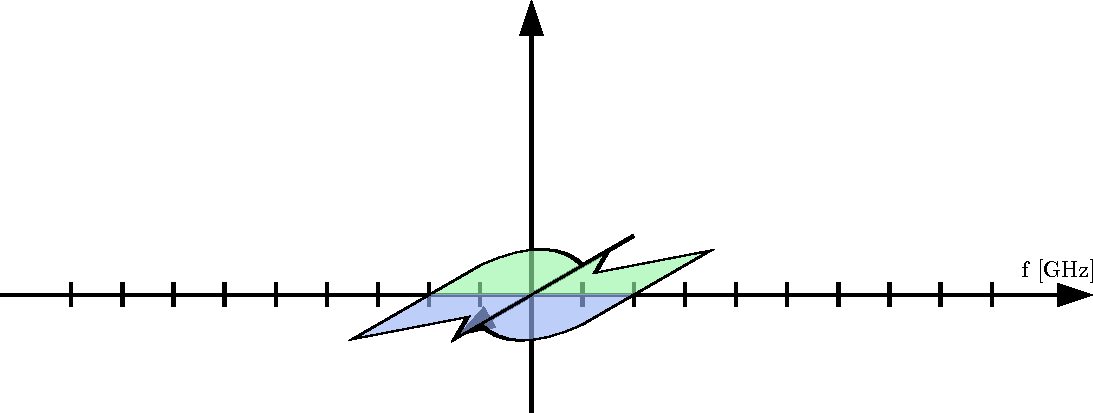
\includegraphics[width=\textwidth]{figures/rx_rf_1_freq_b}
        \vspace{-3mm}
        \[b(t) = \text{LP}\{\mathcal{H}^{-1}\{r\}(t) \cdot \cos(2\pi \cdot f_{\text{RX LO}} \cdot t)\}\]
      \end{column}
    \end{columns}
  }

  \only<3>{
    \vspace{5mm}
    \begin{columns}[T]
      \begin{column}{.5\textwidth}
        {\color{blue} Step 3:}
        \vspace{5mm}
        %todo: ev. border (prio 99)
        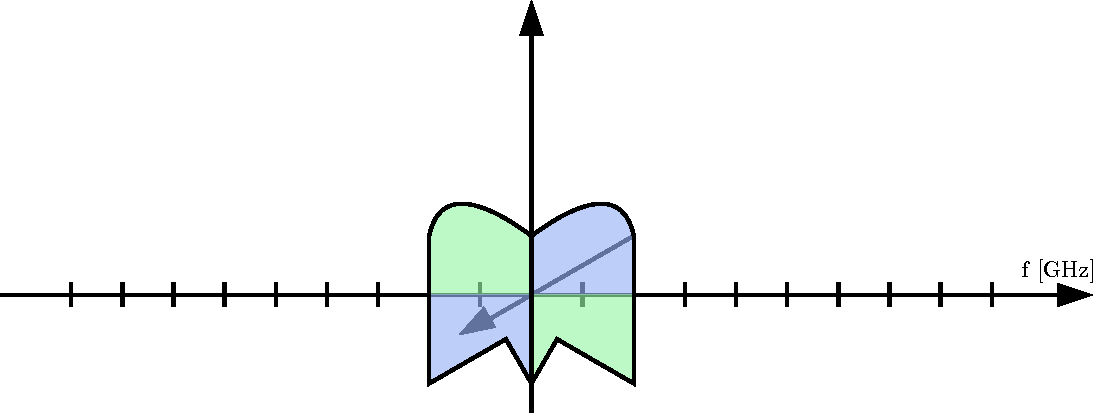
\includegraphics[width=\textwidth]{figures/rx_rf_1_freq_Hb}
        \vspace{-8mm}
        \[\mathcal{H}\{b\}(t)\]
      \end{column}
      \begin{column}{.5\textwidth}
        \vspace{1eM}
        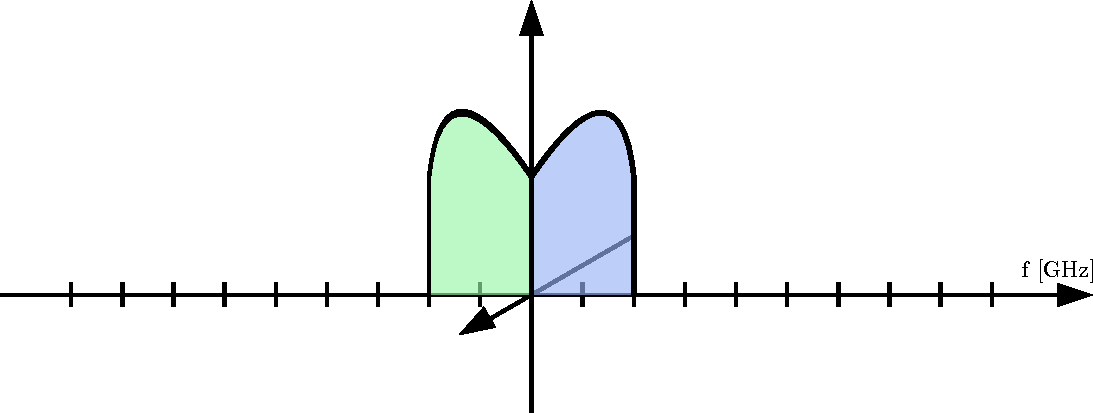
\includegraphics[width=\textwidth]{figures/rx_rf_1_freq_c}
        \vspace{-3mm}
        \[c(t) = a(t) + \mathcal{H}\{b\}(t)\]
      \end{column}
    \end{columns}
  }
\end{frame}

\begin{frame}{Quadrature Intermediate Frequency Sub-Nyquist Sampling}
  \only<1>{
    \centering
    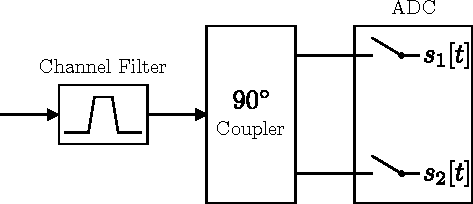
\includegraphics[width=0.6\textwidth]{figures/rx_adc_3_bd}
    \vspace{4mm}
  }

  \only<1-2>{
    \begin{columns}[T]
      \begin{column}{.5\textwidth}
        {\color{blue} Step 1:}
        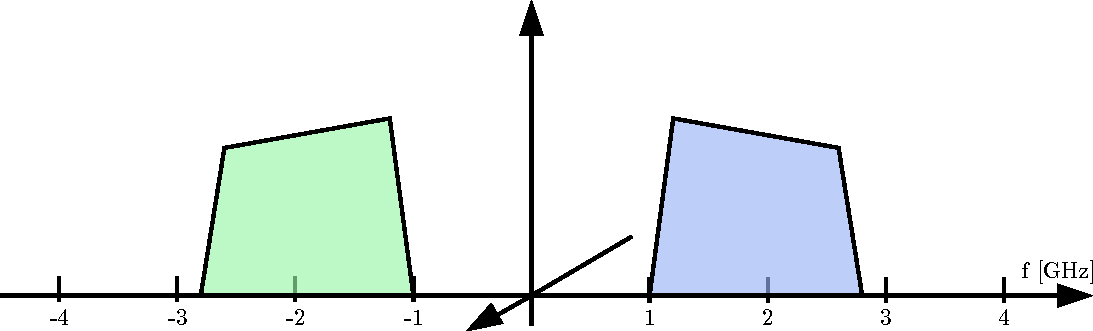
\includegraphics[width=\textwidth]{figures/rx_adc_3_c}
        \vspace{-3mm}
        \[c(t)\]
      \end{column}
      \begin{column}{.5\textwidth}
        \vspace{1eM}
        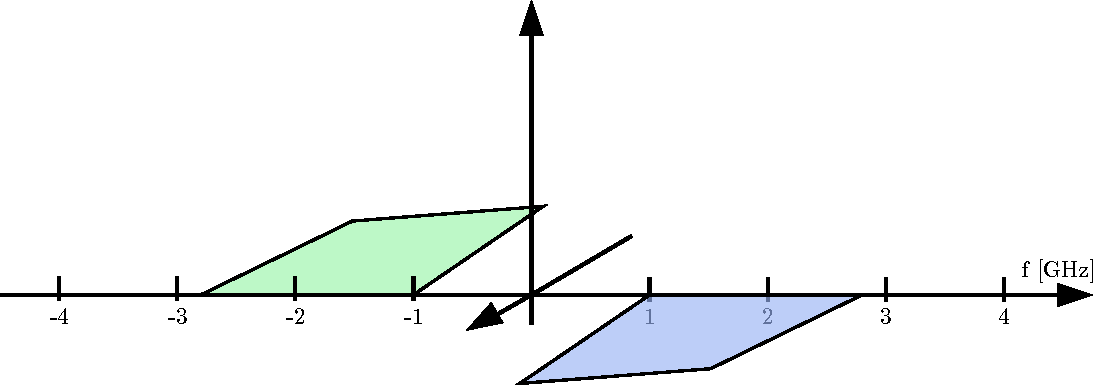
\includegraphics[width=\textwidth]{figures/rx_adc_3_Hc}
        \vspace{-3mm}
        \[\mathcal{H}^{-1}\{c\}(t)\]
      \end{column}
    \end{columns}
  }

  \only<2-3>{
    \vspace{5mm}
    \begin{columns}[T]
      \begin{column}{.5\textwidth}
        {\color{blue} Step 2:}
        \vspace{5mm}
        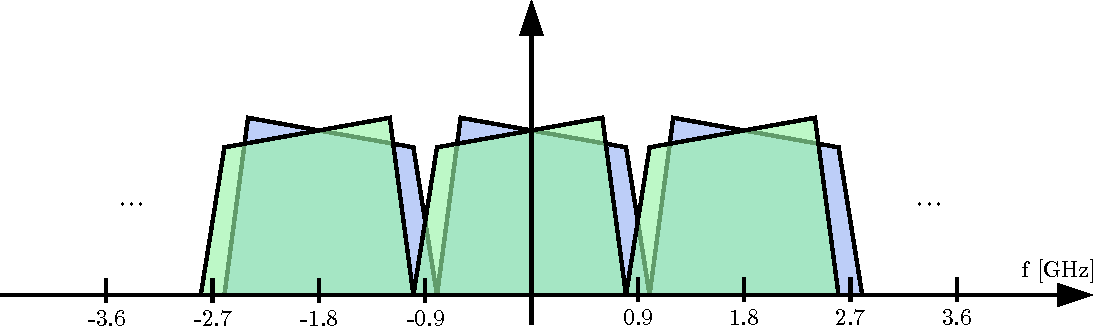
\includegraphics[width=\textwidth]{figures/rx_adc_3_d0}
        \vspace{-8mm}
        \[d_0[k] = c(k/f_s) \]
      \end{column}
      \begin{column}{.5\textwidth}
        \vspace{1eM}
        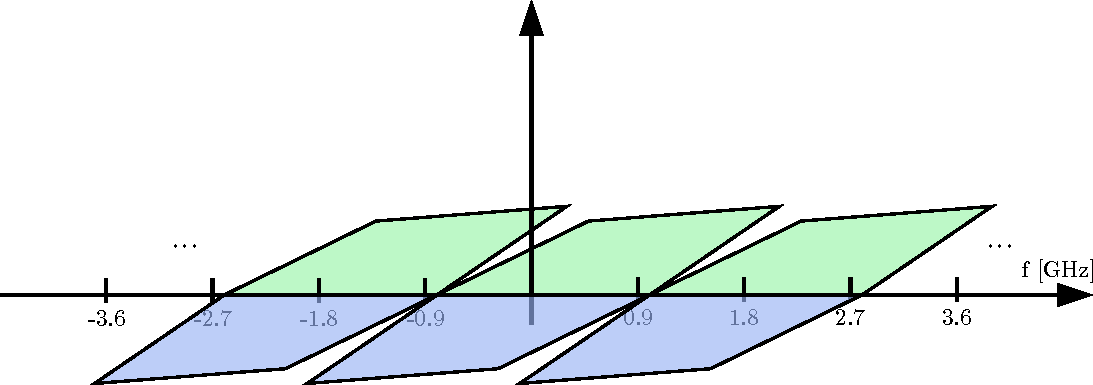
\includegraphics[width=\textwidth]{figures/rx_adc_3_d1}
        \vspace{-3mm}
        \[d_1[k] = \mathcal{H}^{-1}\{c\}(k/f_s)\]
      \end{column}
    \end{columns}
  }

  \only<3-4>{
    \vspace{5mm}
    \begin{columns}[T]
      \begin{column}{.5\textwidth}
        {\color{blue} Step 3:}
        \vspace{5mm}
        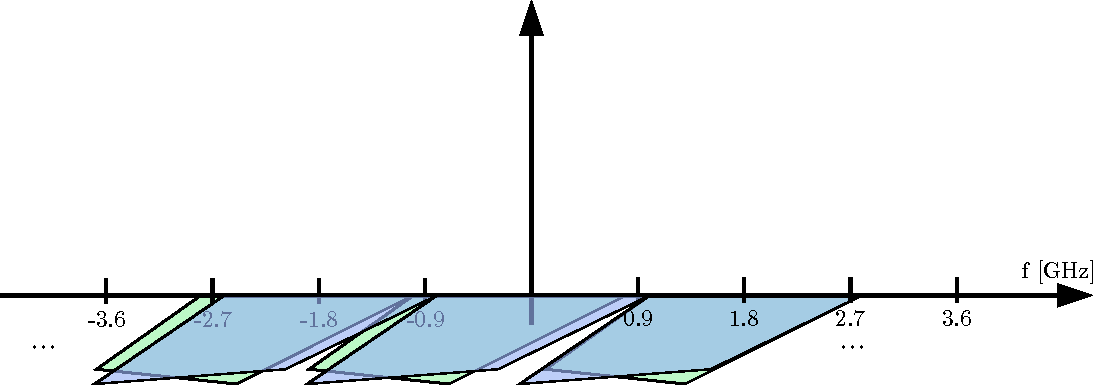
\includegraphics[width=\textwidth]{figures/rx_adc_3_jd0}
        \vspace{-8mm}
        \[j \cdot d_0[k]\]
      \end{column}
      \begin{column}{.5\textwidth}
        \vspace{1eM}
        \vspace{1mm}
        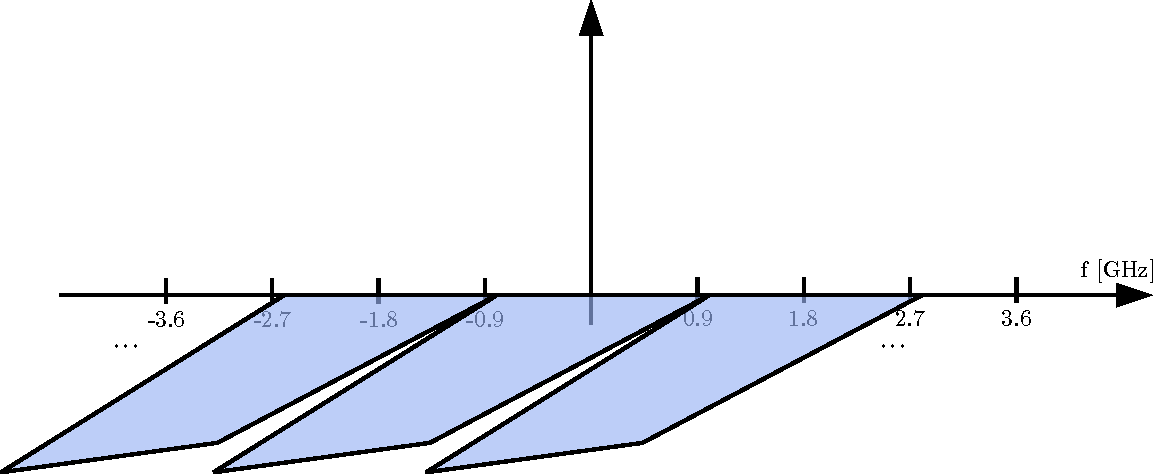
\includegraphics[width=\textwidth]{figures/rx_adc_3_e}
        \vspace{-3mm}
        \[e[k] = d_1[k] + j \cdot d_0[k] \]
      \end{column}
    \end{columns}
  }

  \only<4>{
    \centering
    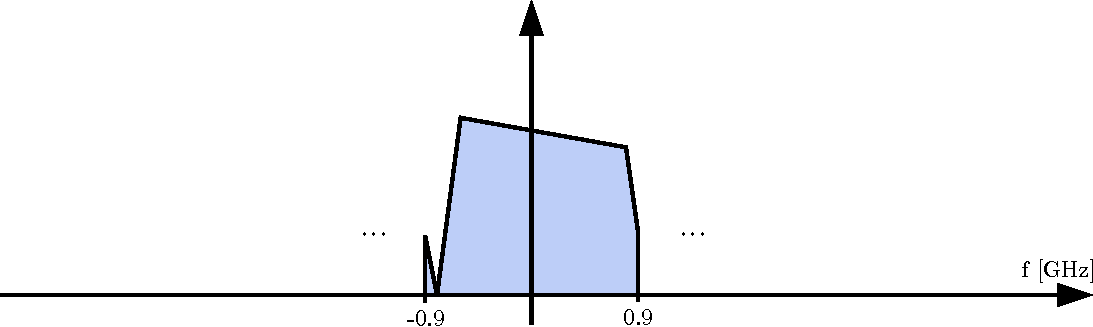
\includegraphics[width=0.5\textwidth]{figures/rx_adc_3_f}
    \vspace{-3mm}
    \[-j \cdot e[k]\]
  }
\end{frame}

\begin{frame}{Digital Acquisition Platform}
  \begin{columns}[T]
    \begin{column}{.5\textwidth}
      \begin{block}{Tasks}
        \begin{enumerate}
        \item Read high resolution samples from ADC
        \item Store data in real-time
        \item Provide download to PC
        \end{enumerate}
      \end{block}
      \vspace{5mm}
      \begin{tikzpicture}
        \node [inner sep=0pt] at (0,0) {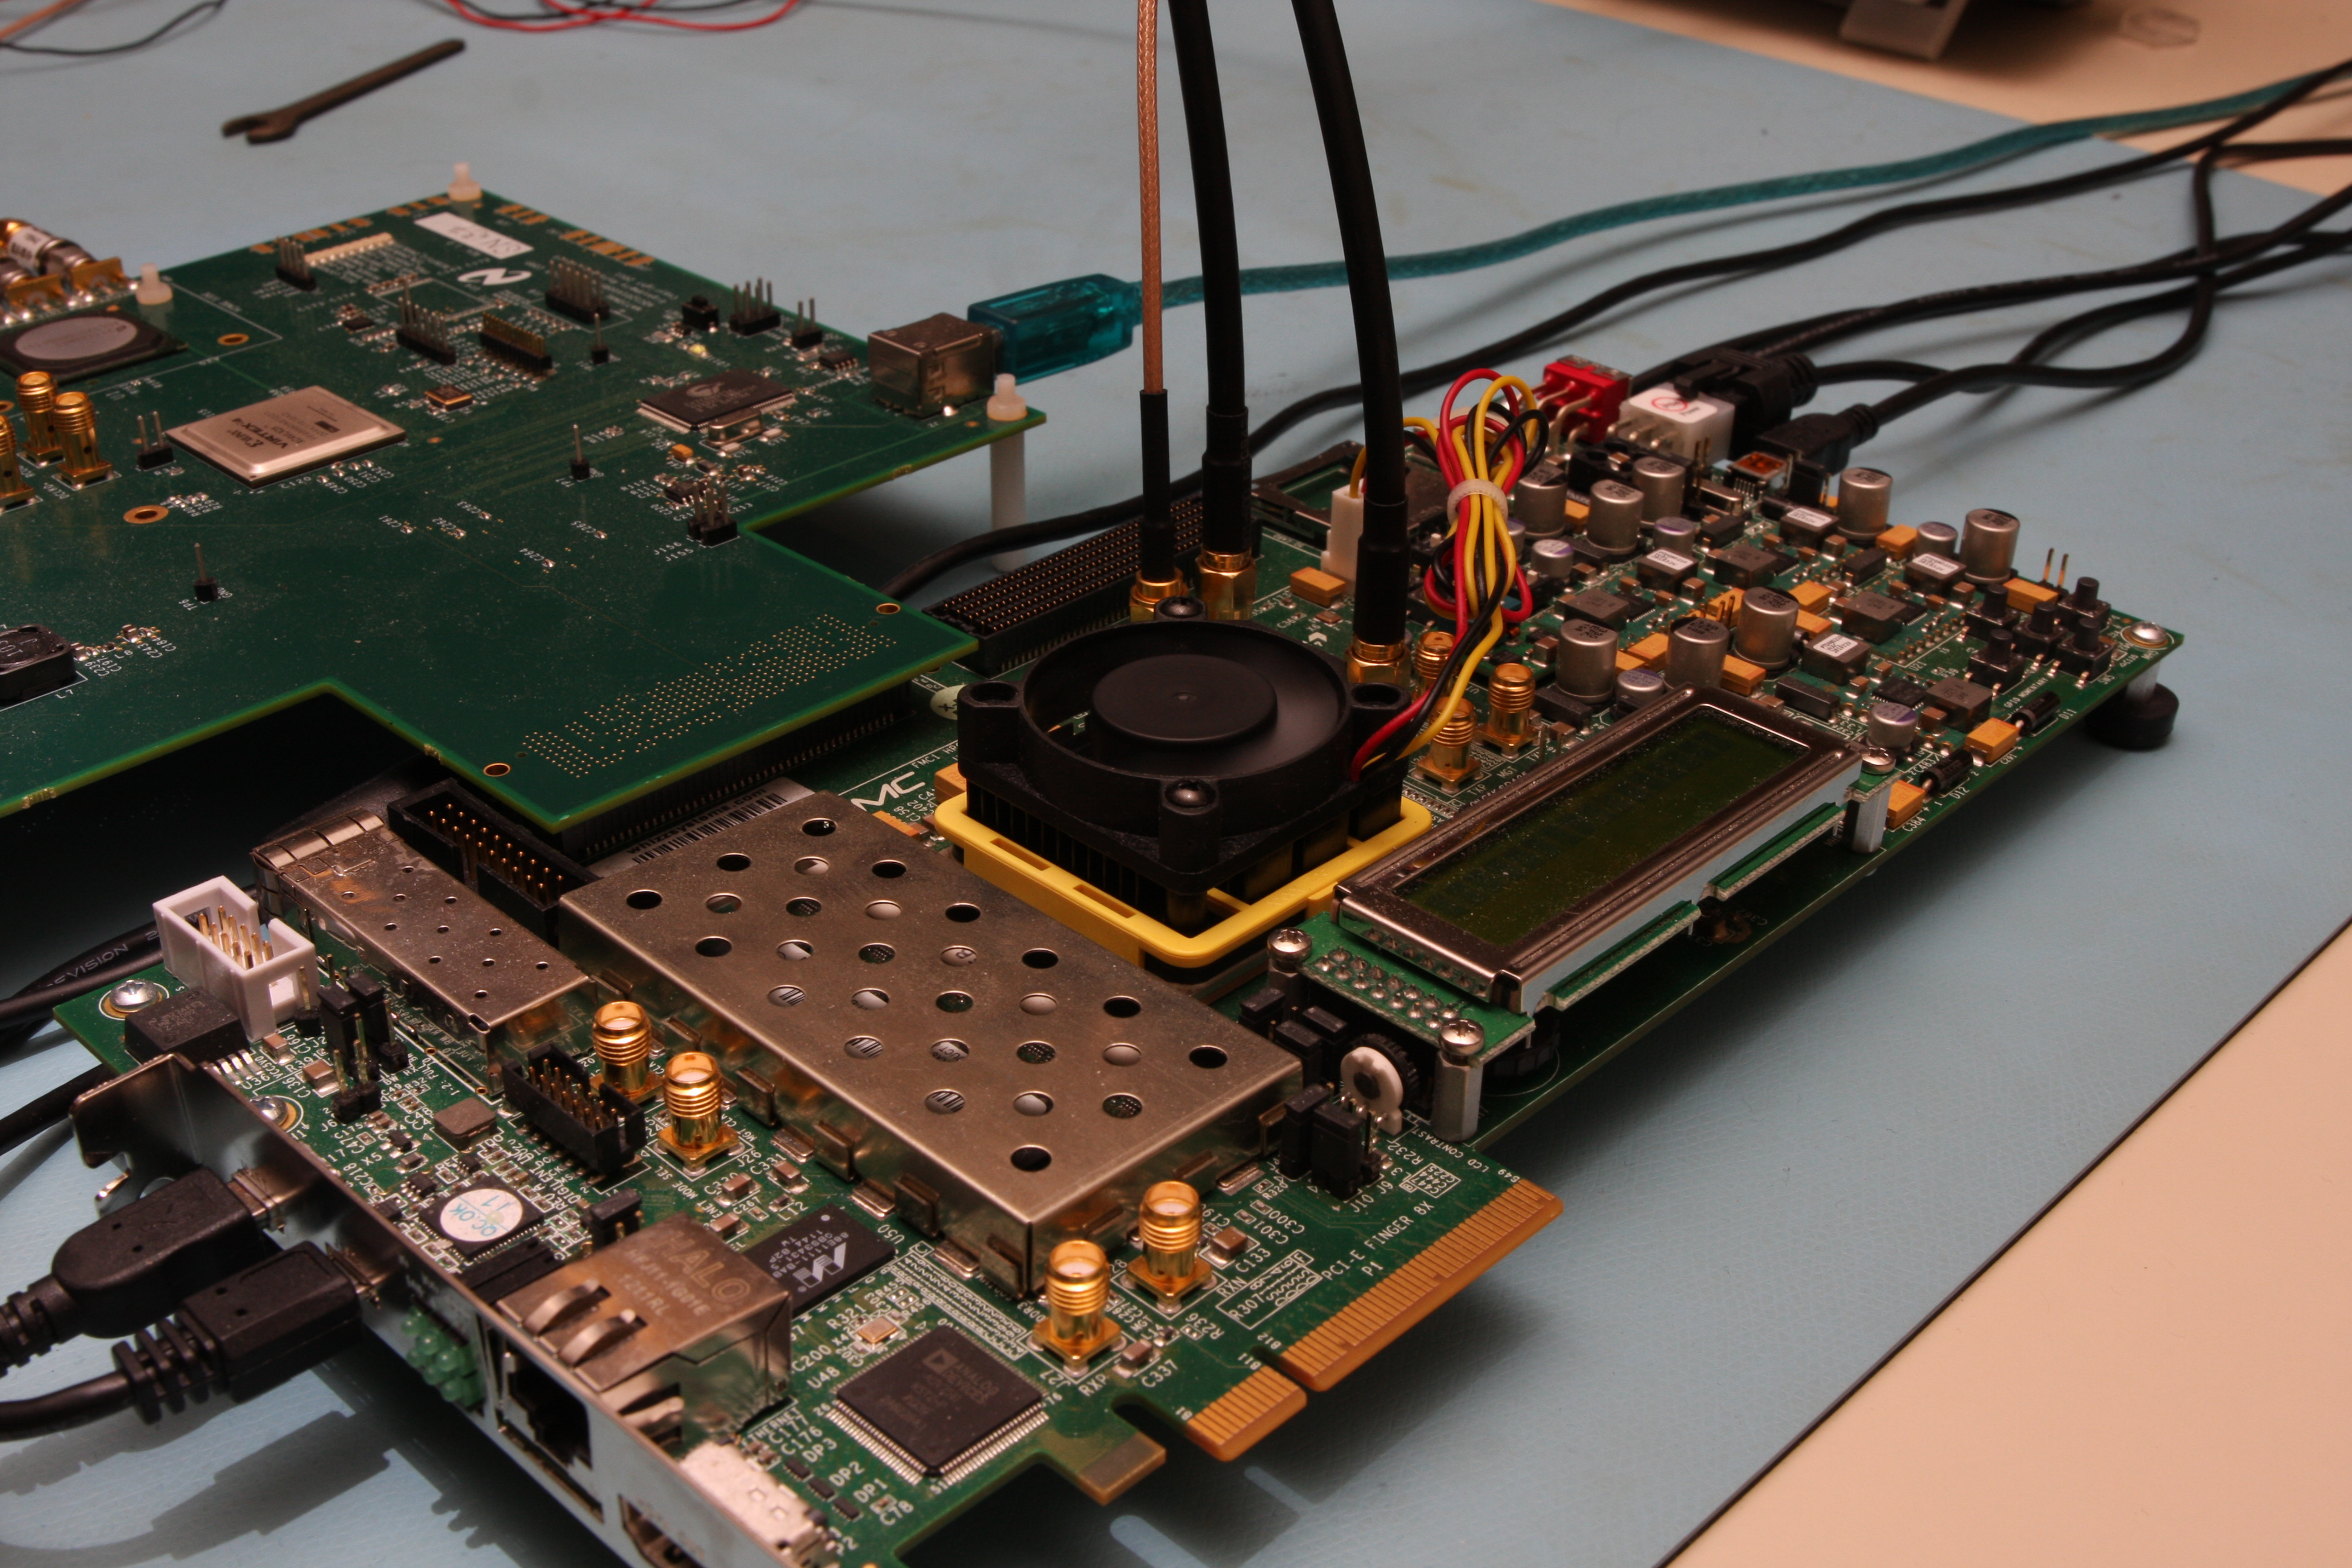
\includegraphics[width=\textwidth]{pictures/fpga}};
        \draw [white, rounded corners=\ClipSep, line width=\ClipSep]
        (current bounding box.north west) --
        (current bounding box.north east) --
        (current bounding box.south east) --
        (current bounding box.south west) -- cycle
        ;
      \end{tikzpicture}
    \end{column}
    \begin{column}{.5\textwidth}
      %todo: optimize color layout
      \begin{block}{Data Storage Speed}
        \begin{itemize}
        \item ADC delivers two 12-bit channels at 1.8 GHz
          $\rightarrow 5.4 \;\text{GB}/\text{s}$.
        \item DDR3 RAM 64 bits at 500 MHz DDR $\rightarrow 8 \;\text{GB}/\text{s}$.
          (P\&R difficult at 800 MHz)
        \end{itemize}
      \end{block}
      \begin{block}{Download Speed}
        \begin{itemize}
        \item USB-to-UART bridge is limited to $1 \text{Mbit}/\text{s}$
          $\rightarrow$ 18 minutes
        \item USB 2.0 can to up to $480 \;\text{Mbit}/\text{s}$, reached speed
          about $140 \;\text{Mbit}/\text{s}$ $\rightarrow$ download in about 1 minute
        \end{itemize}
      \end{block}
    \end{column}
  \end{columns}
\end{frame}

\begin{frame}{FPGA - Architecture}
  % todo: low prio: rename entities
  % ram interface
  % 0-450 MHz
  \only<1>{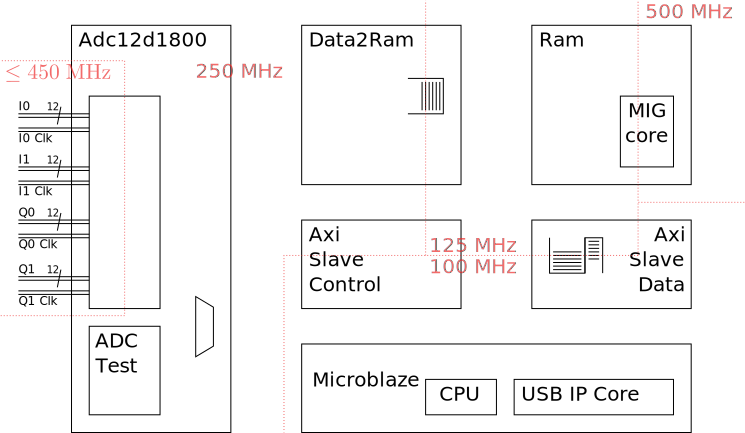
\includegraphics[width=\textwidth]{figures/fpga_architecture_overview}}
  \only<2>{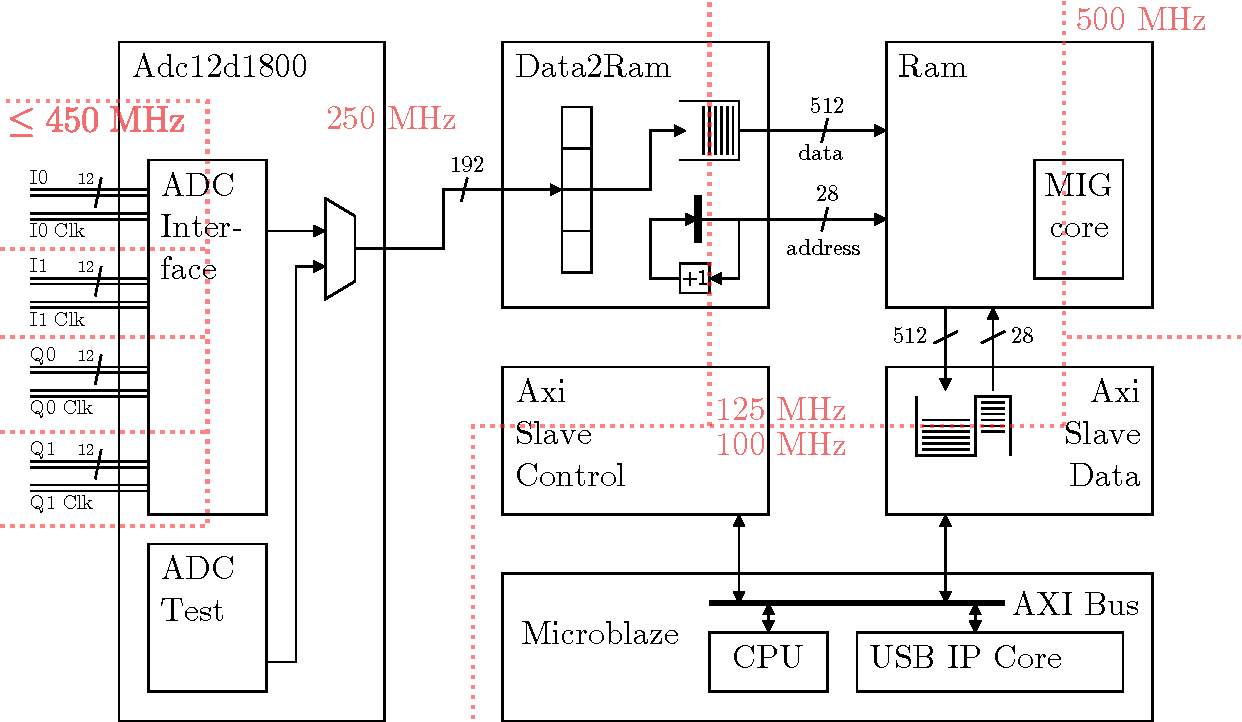
\includegraphics[width=\textwidth]{figures/fpga_clock_domains_overview}}
\end{frame}

\begin{frame}{FPGA - ADC Interface}
  \begin{columns}[T]
    \begin{column}{.7\textwidth}
      \centering
      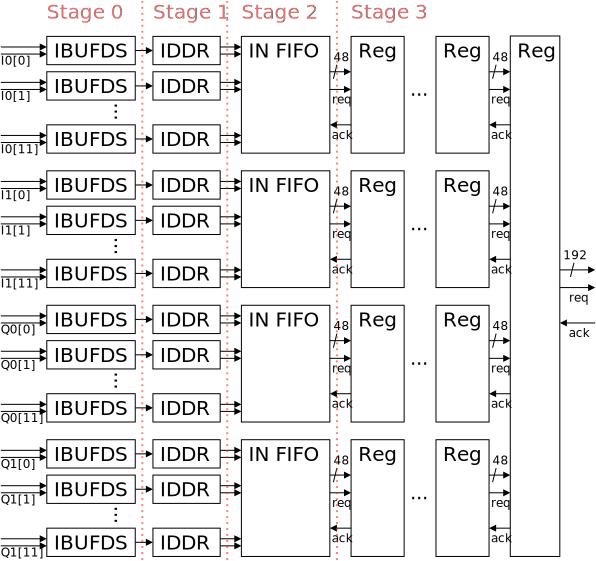
\includegraphics[width=\textwidth]{figures/fpga_adc}
    \end{column}
    \begin{column}{.3\textwidth}
      \begin{block}{Stage 0}
        LVDS to single ended
      \end{block}
      \begin{block}{Stage 1}
        Double to Single Data Rate
      \end{block}
      \begin{block}{Stage 2}
        Clock boundary 450 MHz to 250 MHz
      \end{block}
      \begin{block}{Stage 3}
        Centralization and Reordering
      \end{block}
    \end{column}
  \end{columns}
\end{frame}

\begin{frame}{FPGA - Reset Distribution}
  \begin{columns}[T]
    \begin{column}{.4\textwidth}
      \begin{block}{Challenge}
        Release asynchronous reset accross multiple
        clock domains in same cylce on whole FPGA die
      \end{block}

      \begin{block}{Solution}
        \begin{itemize}
        \item Two global reset trees
        \item Global asynchronous reset
        \item Distributed synchronous deassert
          \begin{itemize}
          \item Local reset Synchronizers
          \item Global 5 MHz reset distribution clock
          \end{itemize}
        \end{itemize}
      \end{block}
    \end{column}
    \begin{column}{.6\textwidth}
      \vspace{6mm}
      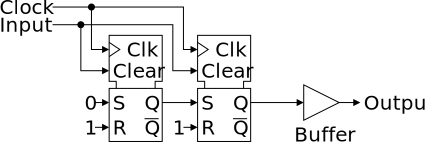
\includegraphics[width=\textwidth]{figures/RstSync} \\
      \vspace{10mm}
      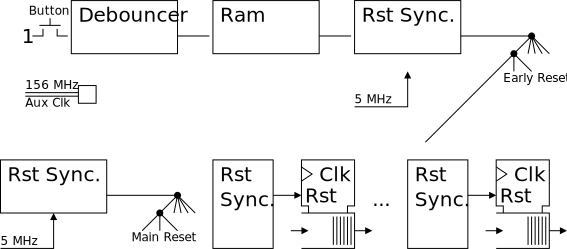
\includegraphics[width=\textwidth]{figures/rst_generation}
    \end{column}
  \end{columns}
\end{frame}

\begin{frame}{Test-Setup}
  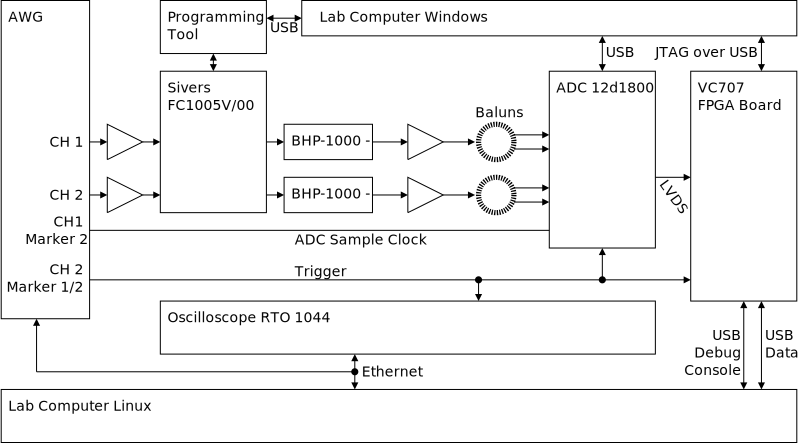
\includegraphics[width=\textwidth]{figures/res_450_setup}
\end{frame}

\begin{frame}{Test-Setup}
  \begin{tikzpicture}
    \node [inner sep=0pt] at (0,0) {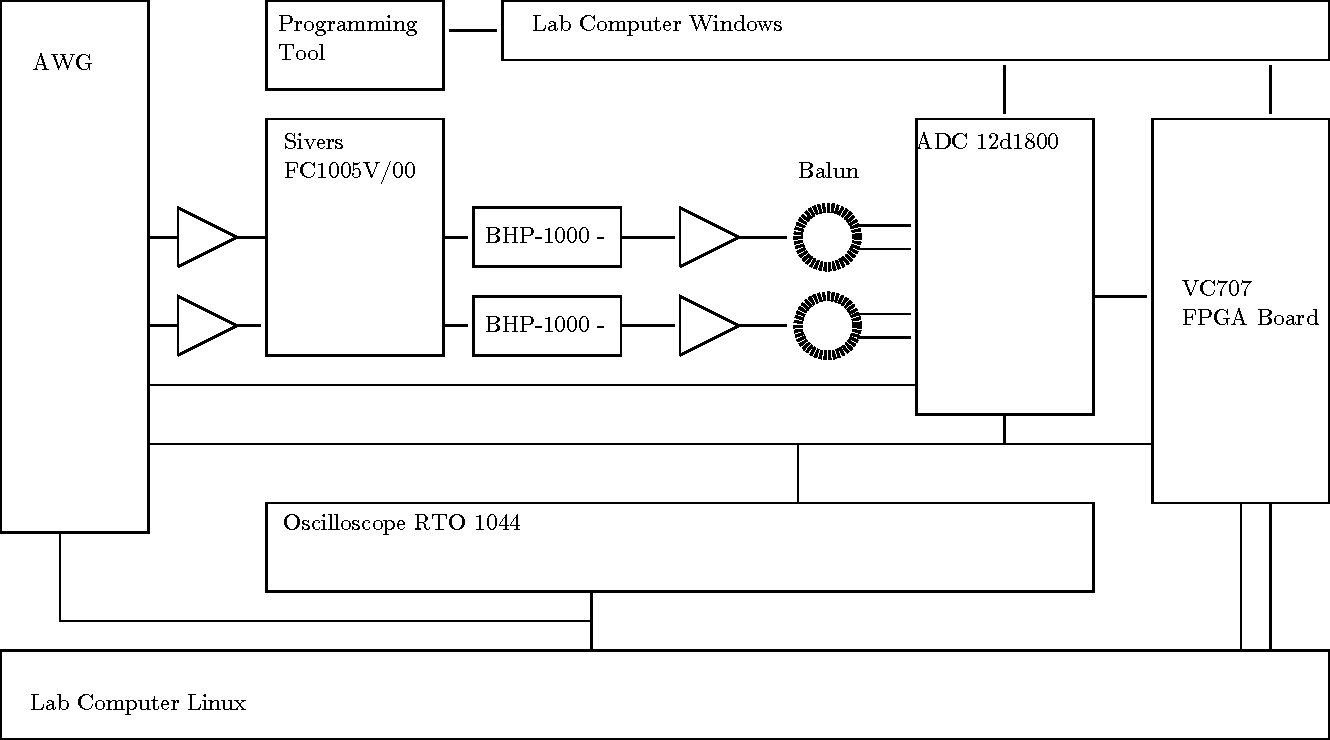
\includegraphics[width=\textwidth]{pictures/res_450_setup}};
    \draw [white, rounded corners=\ClipSep, line width=\ClipSep]
    (current bounding box.north west) --
    (current bounding box.north east) --
    (current bounding box.south east) --
    (current bounding box.south west) -- cycle
    ;
  \end{tikzpicture}
\end{frame}

\begin{frame}{Nyquist-Sampling}
  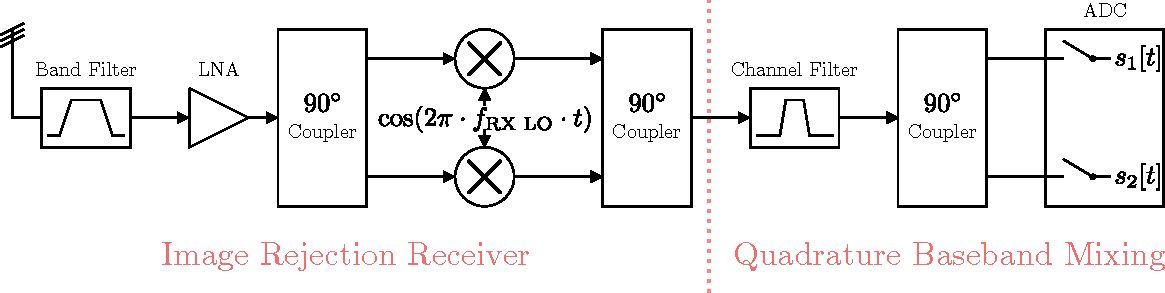
\includegraphics[width=\textwidth]{figures/rx_3_bd} \\

  \begin{columns}[T]
    \begin{column}{.5\textwidth}
      \begin{block}{Setup}
        \begin{tabular}{|l|r@{}l@{~}l|}
          \hline
          $f_{\text{TX IF}}$ & 2&.9&GHz \\ \hline
          $f_{\text{TX LO}}$ & 57&.5&GHz \\ \hline
          $f_{\text{RX LO}}$ & 58&.2&GHz \\ \hline
          $f_{\text{RX IF}}$ & 2&.2&GHz \\ \hline
          Signal Bandwidth B & 0&.45&GHz \\ \hline
          Sample Rate $f_s$ & 1&.8&GHz \\ \hline
        \end{tabular}
      \end{block}
    \end{column}
    \begin{column}{.5\textwidth}
      \begin{block}{Key Points}
        \begin{itemize}
        \item Up to 900 MS/s fits into Nyquist-zone
        \item Performance of $90^\circ$ coupler does not matter
        \end{itemize}
      \end{block}
    \end{column}
  \end{columns}
\end{frame}

\begin{frame}{First Results at 450 MS/s, Phase Noise, Delay Spread}
  \begin{columns}[T]
    \begin{column}{.5\textwidth}
      \centering
      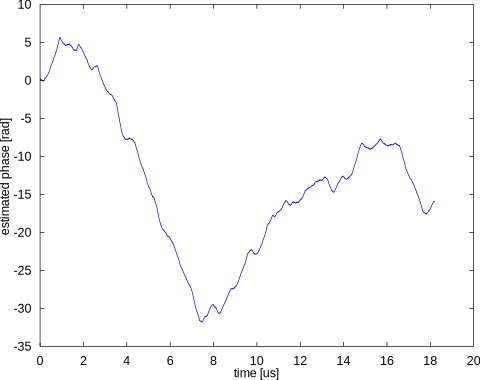
\includegraphics[width=\textwidth]{figures/matlab/res_450_qam4_phase_est} \\
      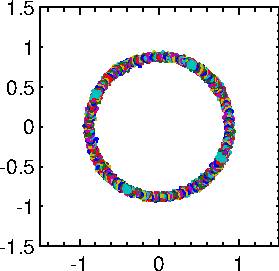
\includegraphics[width=0.6\textwidth]{figures/matlab/res_450_qam4_pnoise} \\
    \end{column}
    \begin{column}{.5\textwidth}
      \centering
      \begin{block}{Time Comparison}
        \begin{description}
        \item[$1 \mu \text{s}$] 1800 symbols @1.8 GS/s
        \item[$2 \mu \text{s}$] CIFS
        \end{description}
      \end{block}

      \begin{block}{Delay Spread}
        98\% of energy
        \begin{description}
        \item[$3$ symobls] @ 450 MS/s
        \item[$10$ symbols] @ 1.8 GS/s
        \end{description}
      \end{block}
    \end{column}
  \end{columns}
\end{frame}

\begin{frame}{450 MS/s Results}
  %todo: db
  \begin{columns}[T]
    \begin{column}{.5\textwidth}
      \only<1>{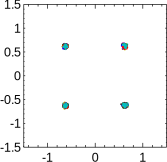
\includegraphics[width=\textwidth]{figures/matlab/res_450_qam4_nice}}
      \only<2>{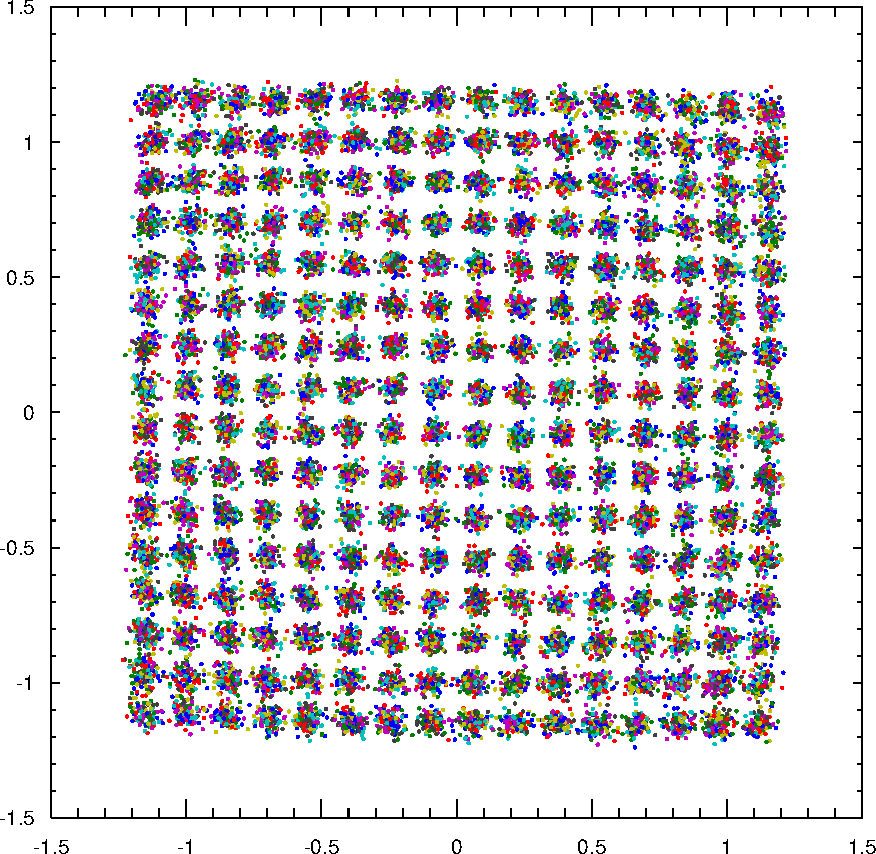
\includegraphics[width=\textwidth]{figures/matlab/res_450_qam256_nice}}
    \end{column}
    \begin{column}{.5\textwidth}
      \begin{block}{Error Vector Magnitude}
        \begin{tabular}{|l|r@{}l|}
          \hline
          Sample rate, system             & \mc{2}{$\text{EVM}_\text{D}$} \\ \hline
          450 MS/s full                   & -26&.57      \\ \hline
        \end{tabular}
      \end{block}
      \begin{block}{450 MS/s full}
        \begin{itemize}
        \item System works
        \item Works up to QAM-256
        \end{itemize}
      \end{block}
      \begin{block}{Raw Data Speed @ 450 MS / s}
        \begin{itemize}
        \item QAM-4: $0.838 \;\frac{\text{GiBit}}{\text{s}}$ \\
        \item QAM-256: $3.353 \;\frac{\text{GiBit}}{\text{s}}$
        \end{itemize}
      \end{block}
    \end{column}
  \end{columns}
\end{frame}

\begin{frame}{1.8 GS/s Results}
  % not full table
  \begin{columns}[T]
    \begin{column}{.5\textwidth}
      \begin{block}{Setup}
        \begin{tabular}{|l|r@{}l@{~}l|}
          \hline
          $f_{\text{TX IF}}$ & 2&.6&GHz \\ \hline
          $f_{\text{TX LO}}$ & 57&.5&GHz \\ \hline
          $f_{\text{RX LO}}$ & 58&.2&GHz \\ \hline
          $f_{\text{RX IF}}$ & 1&.9&GHz \\ \hline
          Signal Bandwidth B & 1&.8&GHz \\ \hline
          Sample Rate $f_s$ & 1&.8&GHz \\ \hline
        \end{tabular}
      \end{block}
      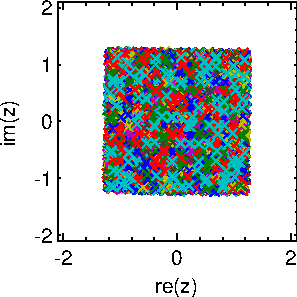
\includegraphics[width=0.6\textwidth]{figures/matlab/res_450_qam256_cp_corr_pcorr_initial}
    \end{column}
    \begin{column}{.5\textwidth}
      \begin{block}{Error Vector Magnitude}
        \begin{tabular}{|l|r@{}l|}
          \hline
          Sample rate, system             & \mc{2}{$\text{EVM}_\text{D}$} \\ \hline
          450 MS/s full                   & -26&.57      \\ \hline
          1.8 GS/s full                   & -16&.94      \\ \hline
        \end{tabular}
      \end{block}
      \begin{block}{1.8 GS/s full}
        \begin{itemize}
        \item Quadrature-Sampling required
        \item EVM drops significately
        \end{itemize}
      \end{block}
    \end{column}
  \end{columns}
\end{frame}

\begin{frame}{Minimalistic Setup}
  \begin{figure}
    \centering
    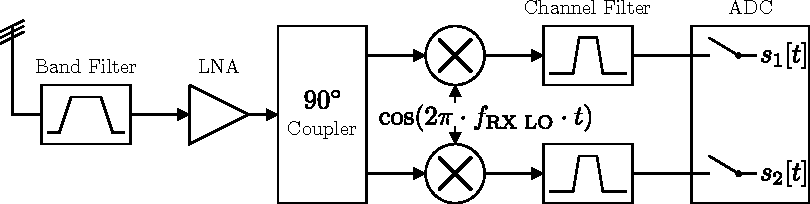
\includegraphics[width=0.7\textwidth]{figures/rx_2_bd}
  \end{figure}

  \begin{columns}[T]
    \begin{column}{.5\textwidth}
      \begin{block}{New Test-Setup}
        \begin{itemize}
        \item Reduce number of components possibly introducing errors
        \item Does not fully suppress other channels
        \item Decreases EVM for 450 MS/s case
        \item Increases EVM for 1.8 GS/s case dramatically
        \end{itemize}
      \end{block}
    \end{column}
    \begin{column}{.5\textwidth}
      \begin{block}{Error Vector Magnitude}
        \begin{tabular}{|l|r@{}l|}
          \hline
          Sample rate, system             & \mc{2}{$\text{EVM}_\text{D}$} \\ \hline
          450 MS/s full                   & -26&.57      \\ \hline
          1.8 GS/s full                   & -16&.94      \\ \hline
          450 MS/s minimal                & {\bf-30}&.29 \\ \hline
          1.8 GS/s minimal                & -7&.73       \\ \hline
        \end{tabular}
      \end{block}
    \end{column}
  \end{columns}
\end{frame}

\begin{frame}{Quadrature Sampling Correction}
  \begin{columns}[T]
    \begin{column}{.5\textwidth}
      \begin{block}{Simple Approach}
        \[c[k] = b[k] + j \cdot \hat a[k]\]
        \[\hat a[k] \;\laplace\; \hat A[k] \]
        \[\hat A[k] = A[k]  \cdot \exp\left(
        \frac{-j}{2 \pi} \left(\frac{\alpha \cdot k}{N} + \beta\right)
        \right)\]
      \end{block}

      \only<1>{
        \begin{tikzpicture}
          \node [inner sep=0pt] at (0,0) {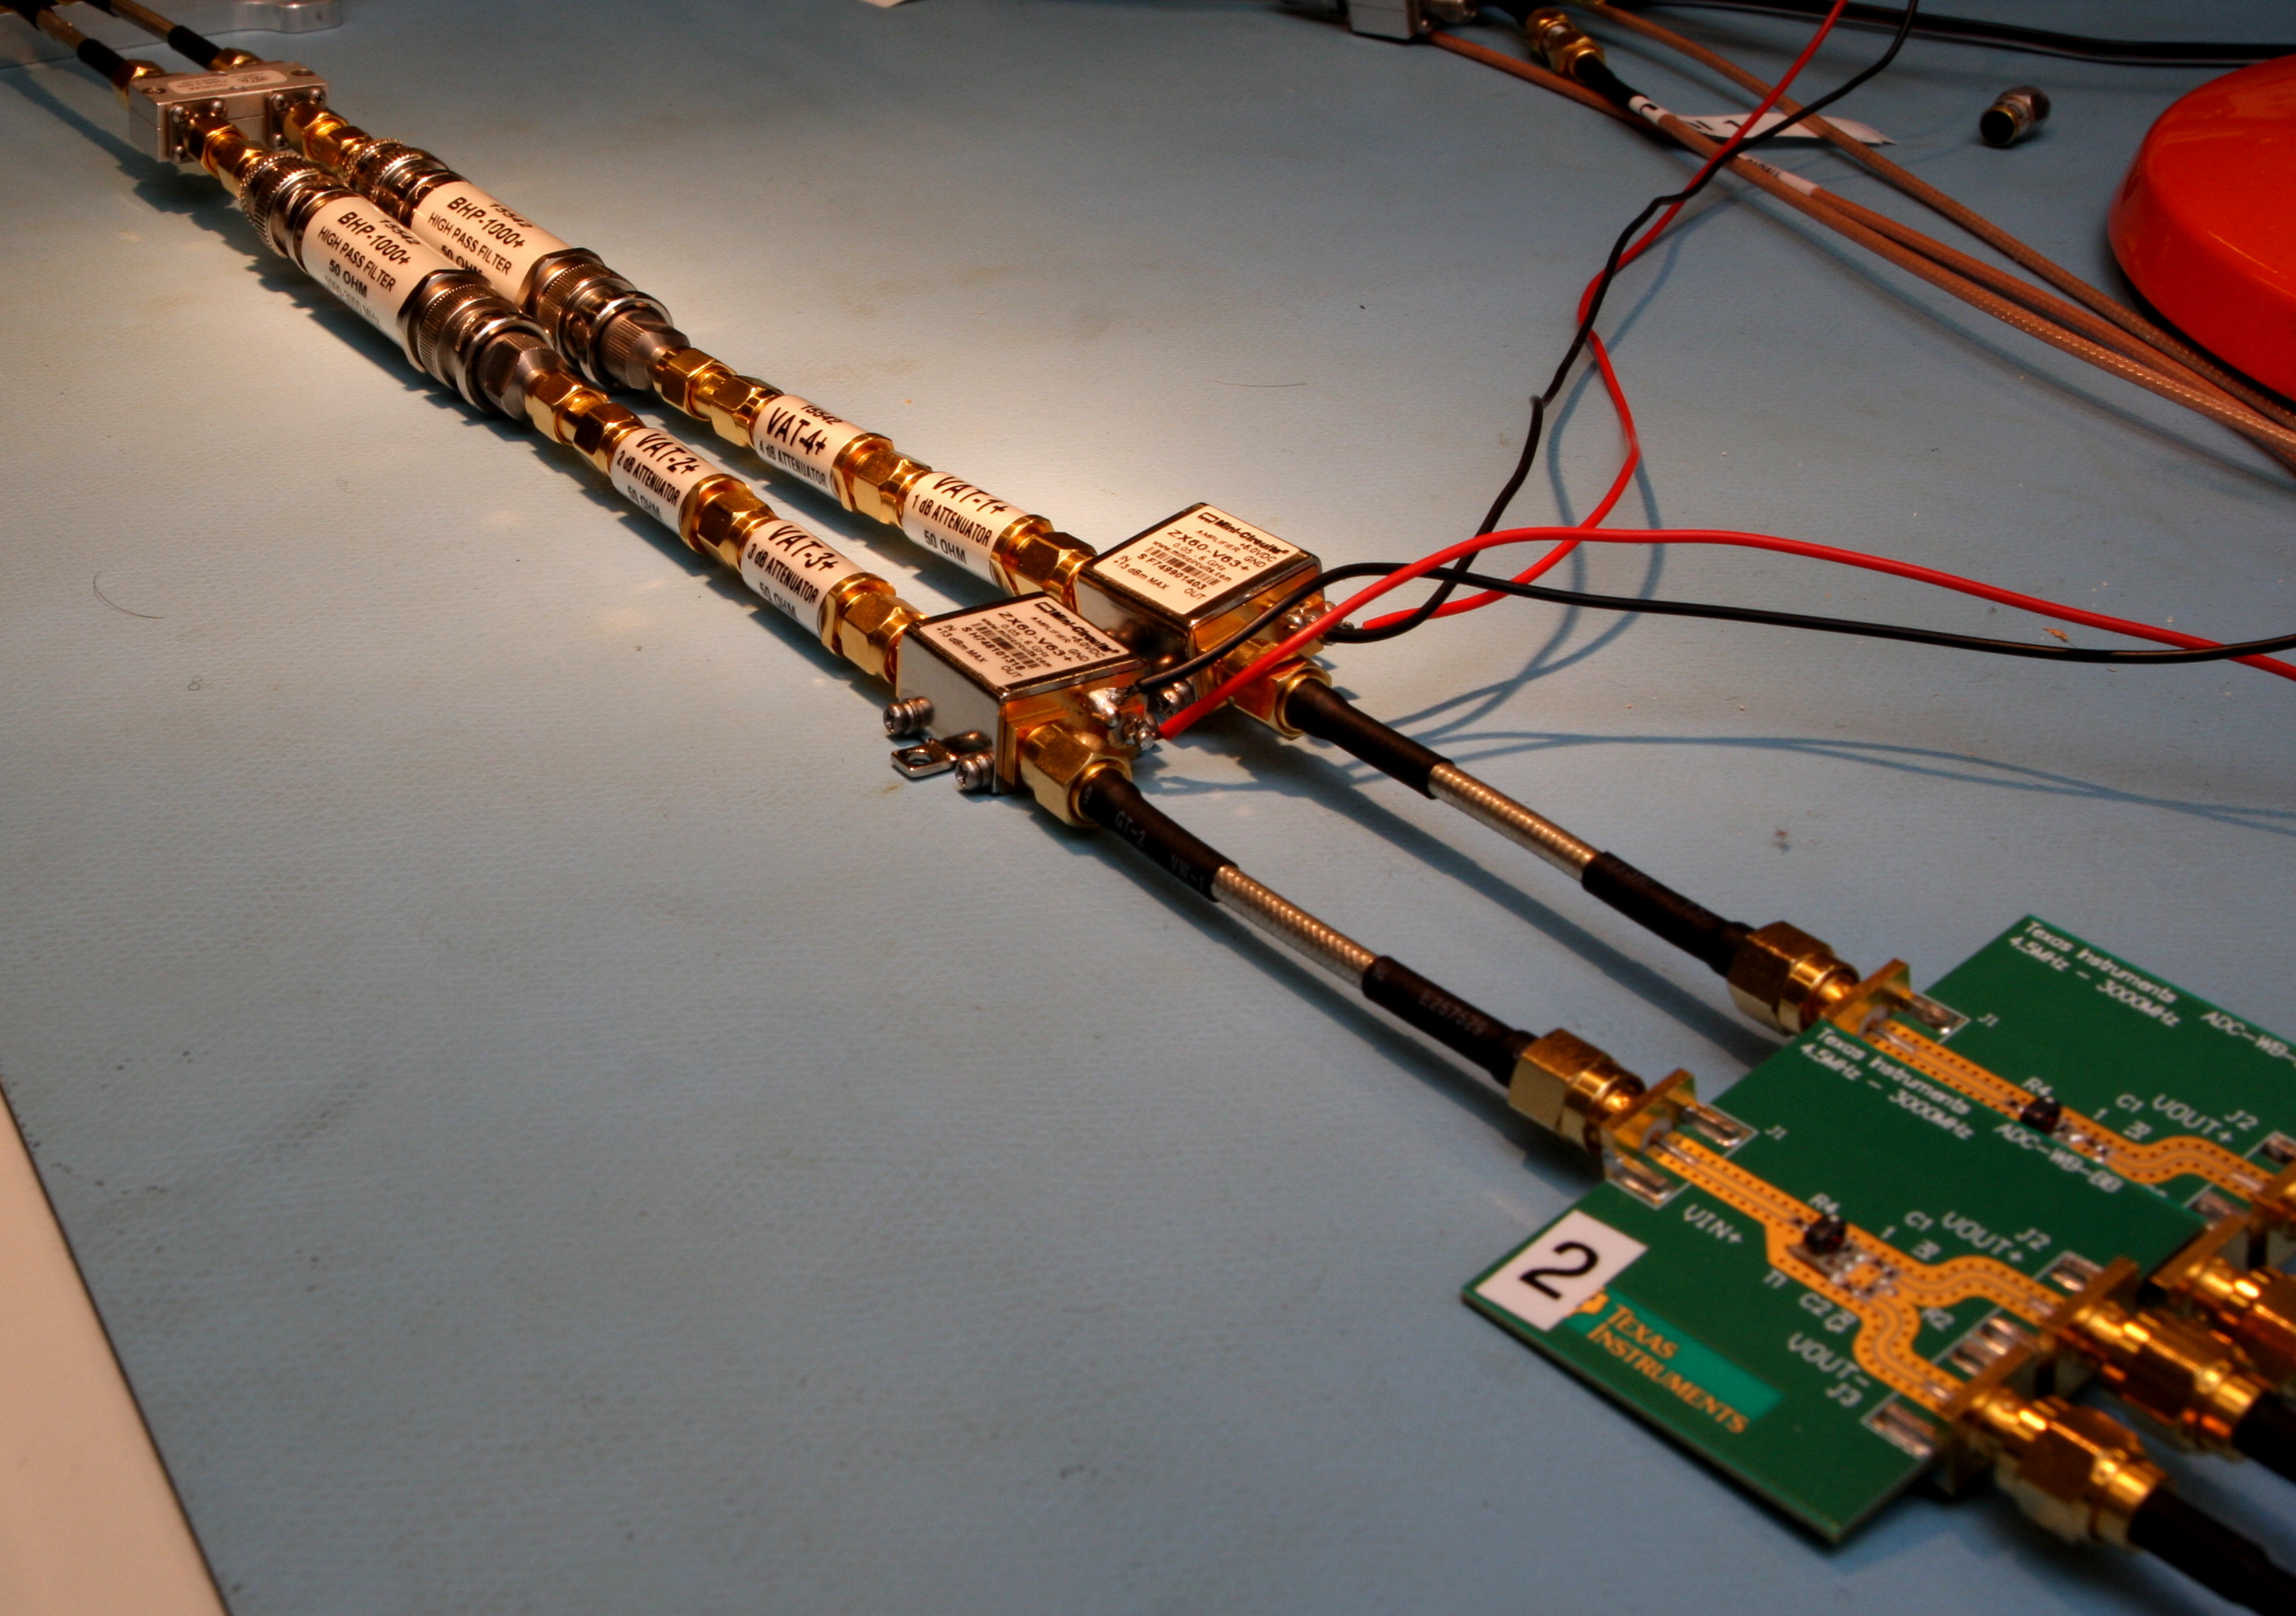
\includegraphics[width=\textwidth]{pictures/filter}};
          \draw [white, rounded corners=\ClipSep, line width=\ClipSep]
          (current bounding box.north west) --
          (current bounding box.north east) --
          (current bounding box.south east) --
          (current bounding box.south west) -- cycle
          ;
        \end{tikzpicture}
      }
      \only<2>{
        \begin{block}{Error Vector Magnitude}
          \begin{tabular}{|l|r@{}l|}
            \hline
            Sample rate, system             & \mc{2}{$\text{EVM}_\text{D}$} \\ \hline
            450 MS/s minimal                & {\bf-30}&.29 \\ \hline
            1.8 GS/s minimal                & -7&.73       \\ \hline
            1.8 GS/s minimal, $\alpha\beta$ & -16&.04      \\ \hline
          \end{tabular}
        \end{block}
      }
    \end{column}
    \begin{column}{.5\textwidth}
      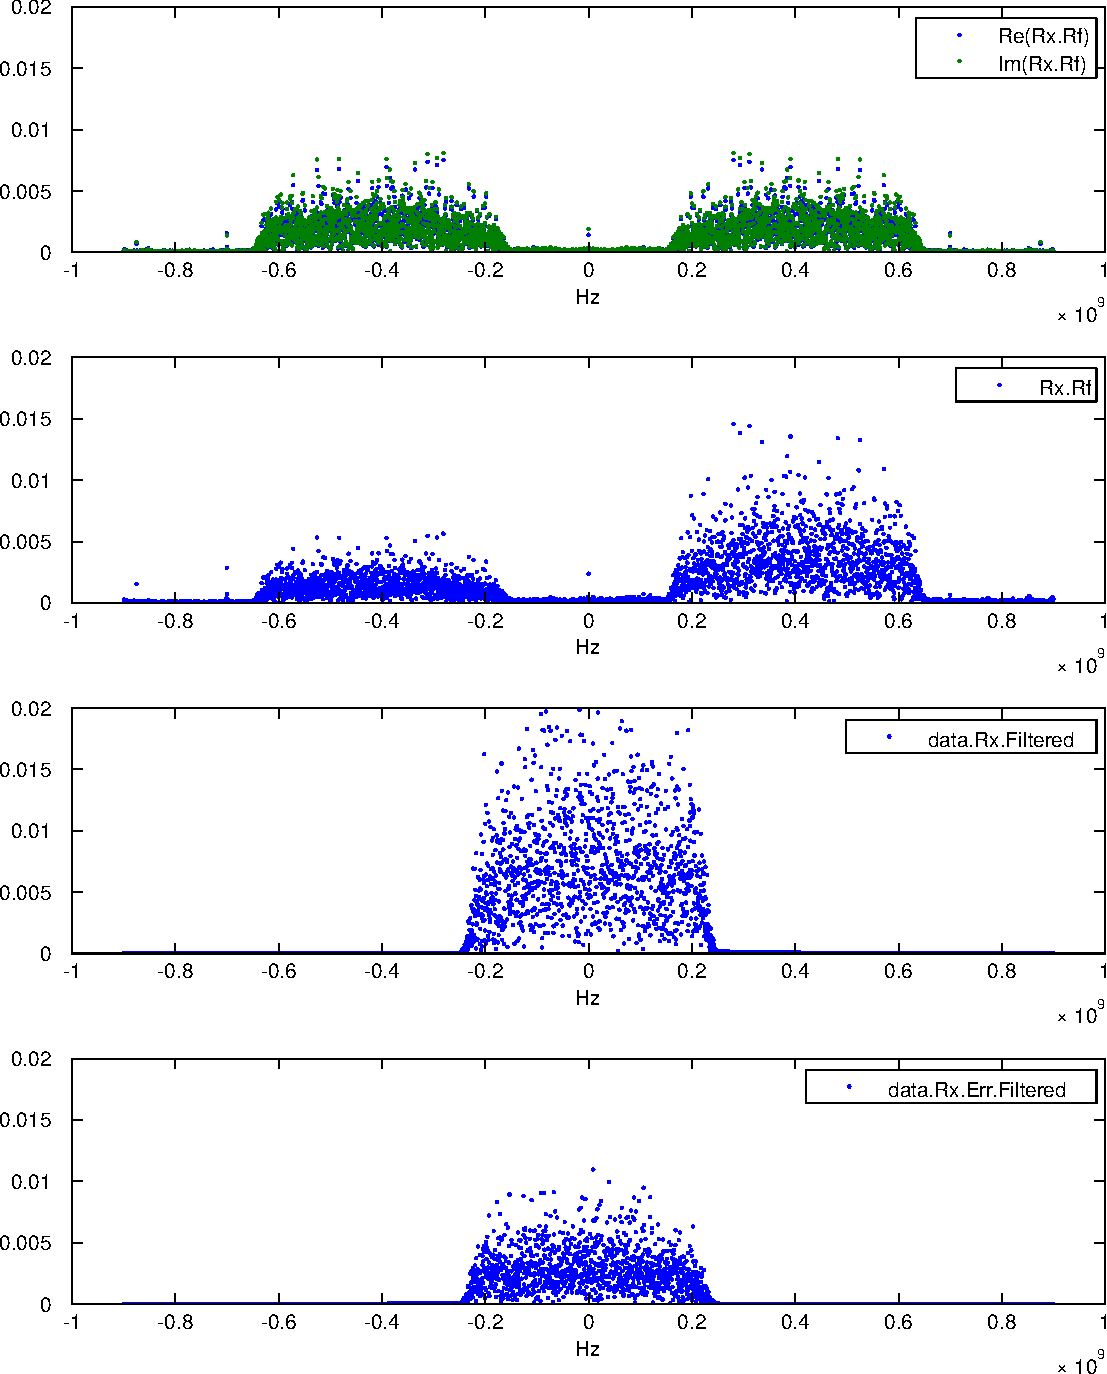
\includegraphics[width=\textwidth]{figures/matlab/res_450_rx_freq}
    \end{column}
  \end{columns}
\end{frame}

\begin{frame}{Quadrature Sampling Correction}
  \begin{columns}[T]
    \begin{column}{.5\textwidth}
      \begin{block}{Signal Theory Approach}
        \[s_{\text{sig}}[k] = (s[k] + j \mathcal{H}\{s\}[k])/2 \]
        \[s_{\text{err}}[k] = (s[k] - j \mathcal{H}\{s\}[k])/2 \]
        \[s_{\text{sig, mirr}}[k] = s_{\text{sig}}^*[k]\]
        \[c[m] = \sum_k s_{\text{sig, mirr}}[k+m] \cdot s_{\text{Err}}[k] \]
        \[C = \frac{\sup_m c[m]}{\sum_k |s_{\text{sig}}[k]|^2}\]

        \[s_{\text{corr}}[k] = s[k] - (s^*[k] .* C^*)\]
      \end{block}
    \end{column}
    \begin{column}{.5\textwidth}
      \only<1>{
        \includegraphics[width=\textwidth]{figures/matlab/analyzeLsb}
      }
      \only<2>{
        \begin{block}{Error Vector Magnitude}
          \begin{tabular}{|l|r@{}l|}
            \hline
            Sample rate, system             & \mc{2}{$\text{EVM}_\text{D}$} \\ \hline
            450 MS/s full                   & -26&.57      \\ \hline
            1.8 GS/s full                   & -16&.94      \\ \hline
            450 MS/s minimal                & {\bf-30}&.29 \\ \hline
            1.8 GS/s minimal                & -7&.73       \\ \hline
            1.8 GS/s minimal, $\alpha\beta$ & -16&.04      \\ \hline
            1.8 GS/s minimal, xcorr         & -17&.42      \\ \hline
          \end{tabular}
        \end{block}
      }
    \end{column}
  \end{columns}
\end{frame}

\begin{frame}{Conclusion for 60 GHz}
  \begin{columns}[T]
    \begin{column}{.6\textwidth}
      \begin{itemize}
      \item FPGA prototyping is possible
      \item Hardware impairment correction is crucial
      \item High Modulation orders are possible
      \item Sub-Nyquist Sampling reduces analog receiver complexity
      \item Quadrature Sub-Nyquist Sampling gives even more flexibility
      \end{itemize}
    \end{column}
    \begin{column}{.4\textwidth}
      \begin{tikzpicture}
        \node [inner sep=0pt] at (0,0)
              {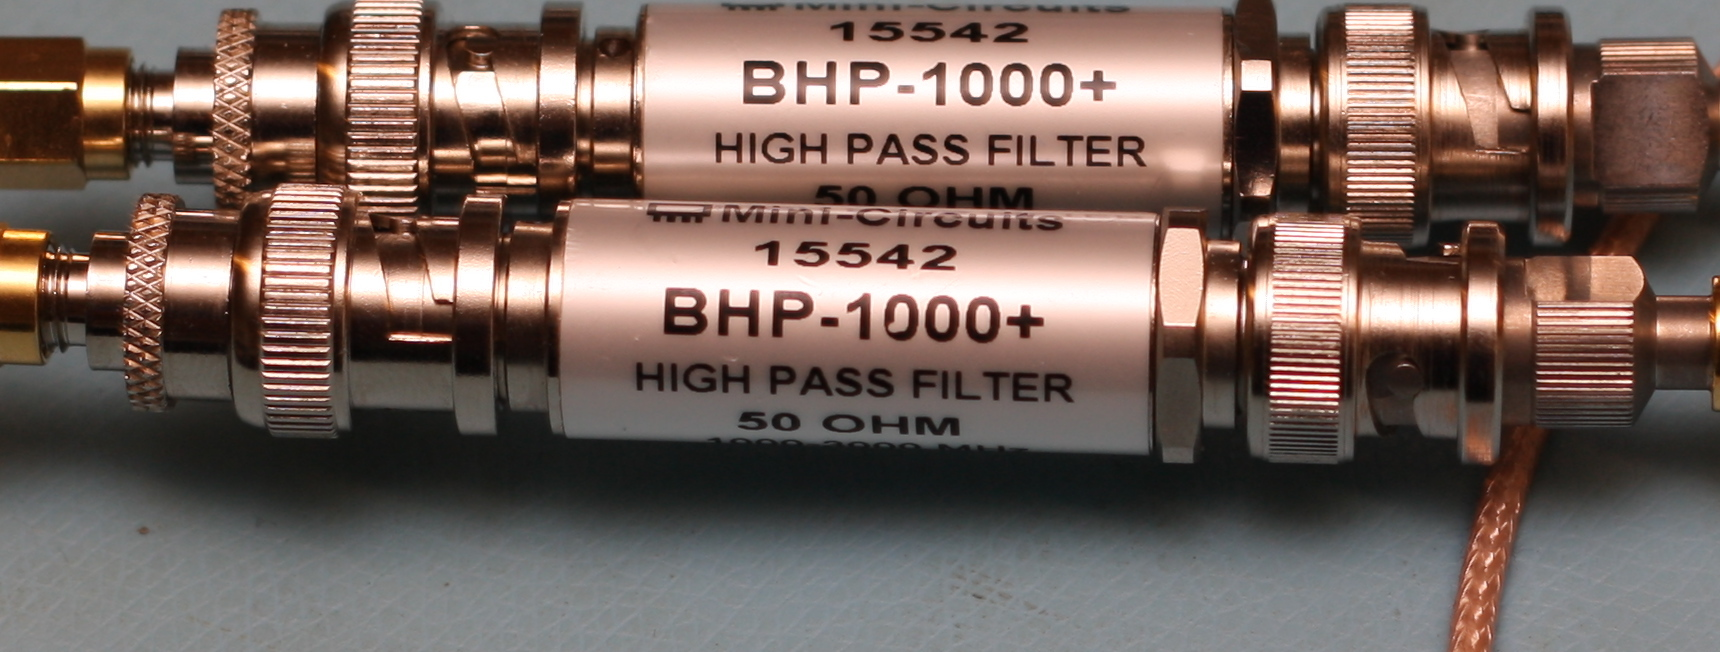
\includegraphics[width=\textwidth]{pictures/BHP-1000+}};
              \draw [white, rounded corners=\ClipSep, line
                width=\ClipSep] (current bounding box.north west) --
              (current bounding box.north east) -- (current bounding
              box.south east) -- (current bounding box.south west) --
              cycle ;
      \end{tikzpicture}
      \begin{tikzpicture}
        \node [inner sep=0pt] at (0,0)
              {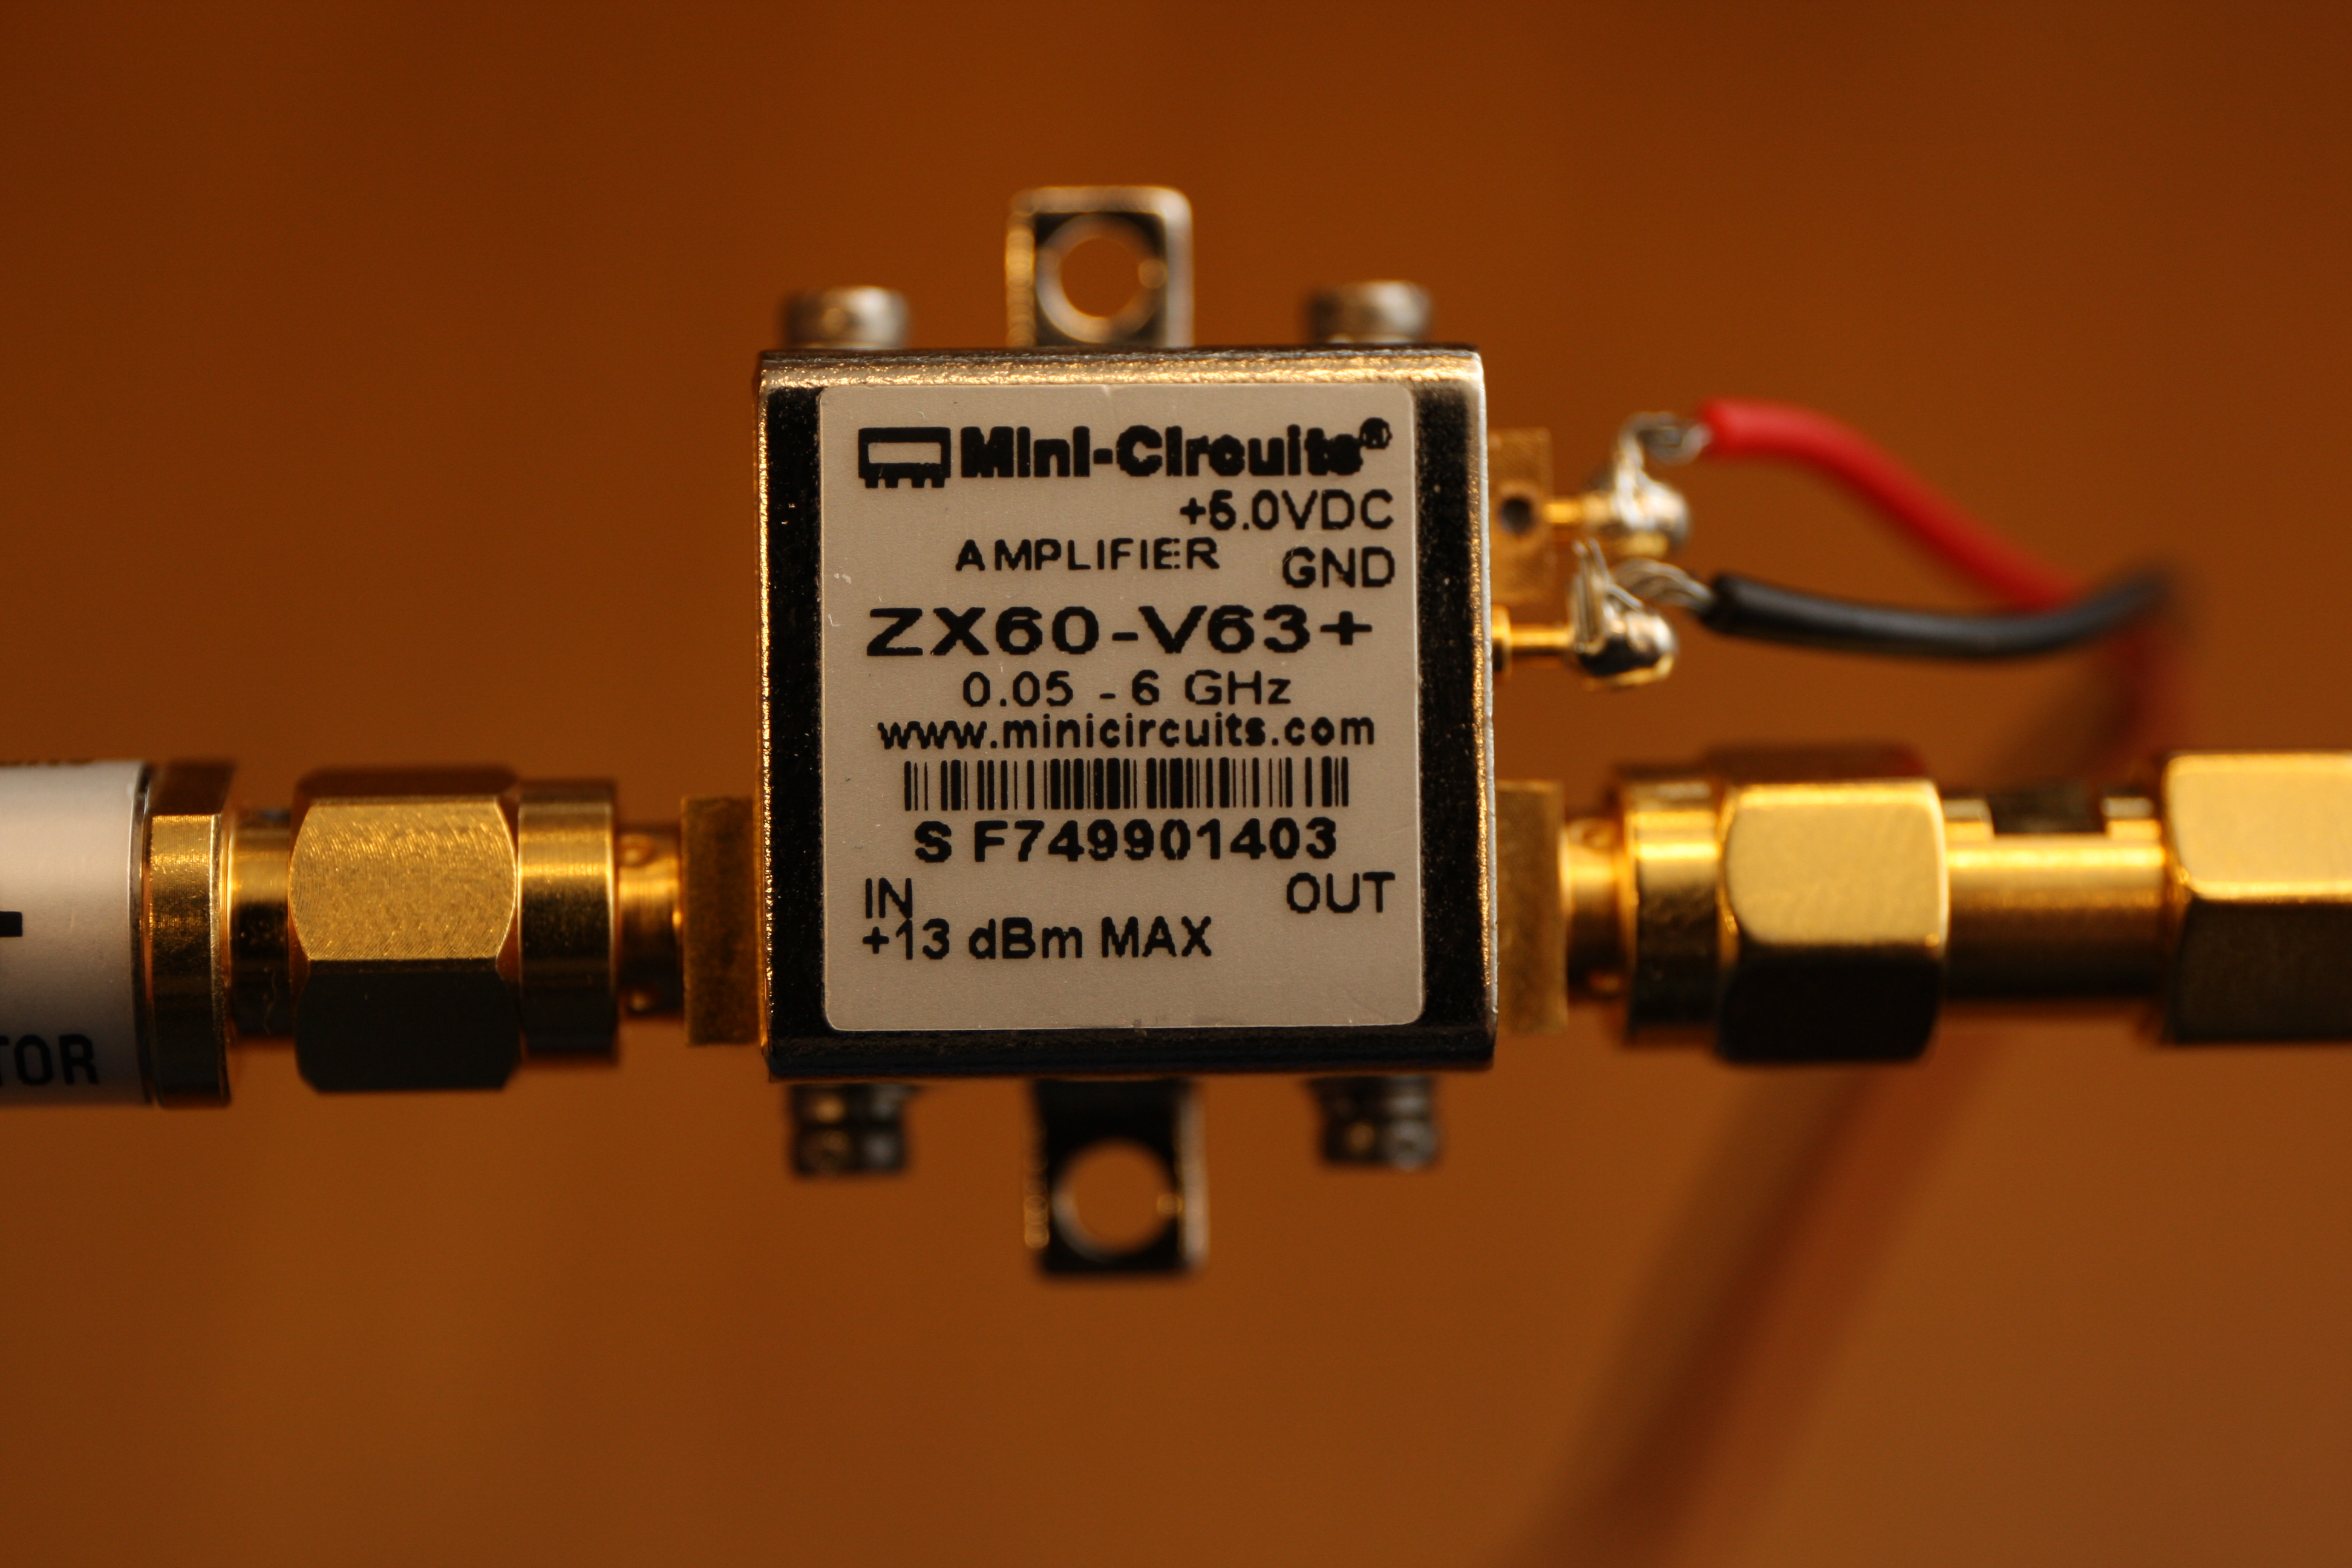
\includegraphics[width=\textwidth]{pictures/ZX60-V63+}};
              \draw [white, rounded corners=\ClipSep, line
                width=\ClipSep] (current bounding box.north west) --
              (current bounding box.north east) -- (current bounding
              box.south east) -- (current bounding box.south west) --
              cycle ;
      \end{tikzpicture}
    \end{column}
  \end{columns}
\end{frame}

\begin{frame}{Outlook}

  \begin{columns}[T]
    \begin{column}{.6\textwidth}
      \begin{itemize}
      \item Use high analog bandwidth of Oscilloscope to Nyquist-sample at 1.8 GS/s
      \item Independent I/Q channel measurement using multiple sine waves
      \item Independent I/Q channel correction
      \item Framework can be used for further simulations
      \item FPGA can be extended
      \end{itemize}
    \end{column}
    \begin{column}{.4\textwidth}
      \begin{tikzpicture}
        \node [inner sep=0pt] at (0,0) {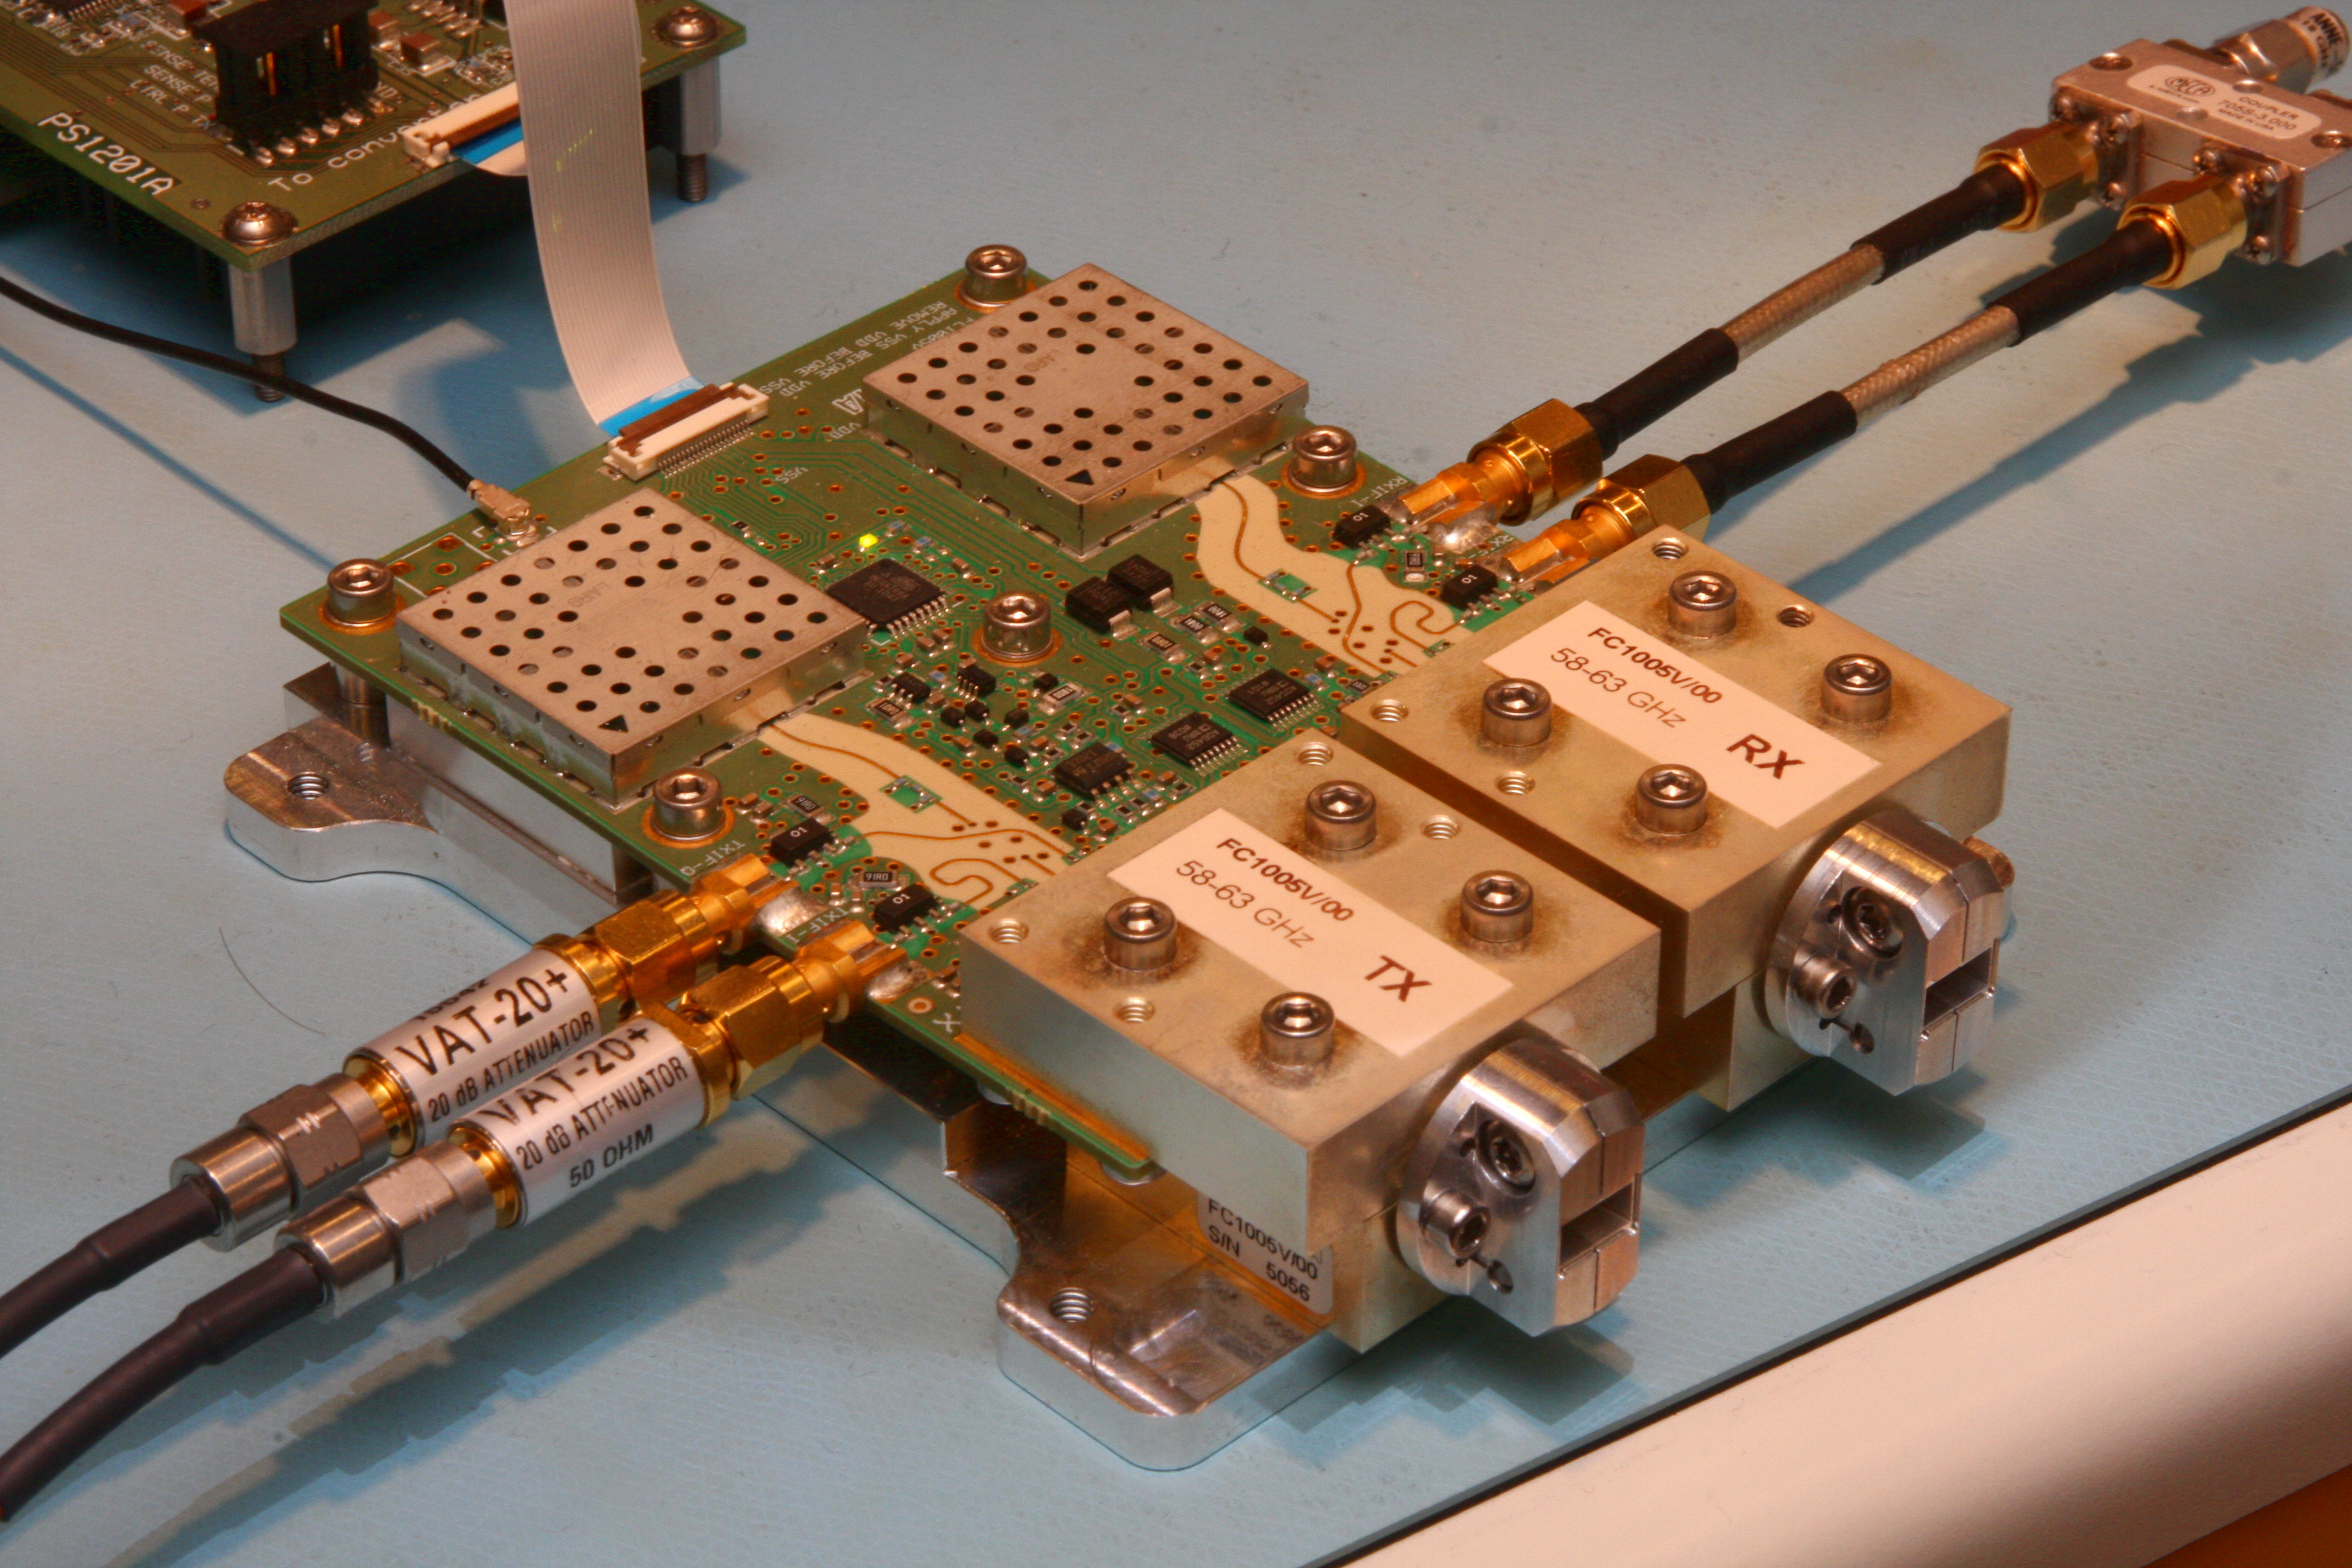
\includegraphics[width=\textwidth]{pictures/sivers}};
        \draw [white, rounded corners=\ClipSep, line width=\ClipSep]
        (current bounding box.north west) --
        (current bounding box.north east) --
        (current bounding box.south east) --
        (current bounding box.south west) -- cycle
        ;
      \end{tikzpicture}
    \end{column}
  \end{columns}
  \vspace{8mm}
  \centering
  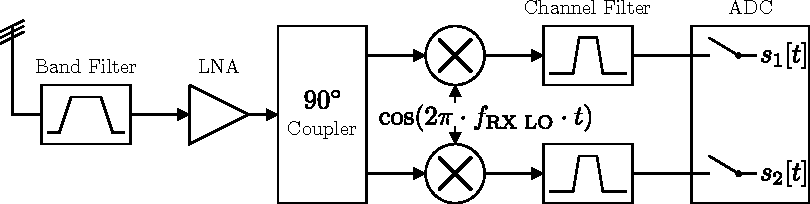
\includegraphics[width=0.7\textwidth]{figures/rx_2_bd} \\
\end{frame}

\begin{frame}[noframenumbering]{Backup: Frame Structure}
  \begin{figure}
    \centering
    \includegraphics[width=0.7\textwidth]{figures/frame_struct}
  \end{figure}

  \begin{figure}
    \centering
    \begin{tabular}{|c|c|c|}
      \hline
      Modulation of Data Fiels & QAM-4 & QAM-256 \\ \hline
      Modulation of Estimation Fields & \mc{2}{BPSK} \\ \hline
      Length of FES field & \mc{2}{256 symbols} \\ \hline
      Length of CES field & \mc{2}{1152 symbols} \\ \hline
      Length of PES field & \mc{2}{32 symbols} \\ \hline
      Length of Data Block & \mc{2}{147 symbols} \\ \hline
      Length of Data Field & \mc{2}{115 symbols} \\ \hline
      Length of Data Field & 230 bits & 920 bits \\ \hline
    \end{tabular}
  \end{figure}
\end{frame}

\end{document}
